% Options for packages loaded elsewhere
\PassOptionsToPackage{unicode}{hyperref}
\PassOptionsToPackage{hyphens}{url}
%
\documentclass[
]{article}
\usepackage{amsmath,amssymb}
\usepackage{lmodern}
\usepackage{iftex}
\ifPDFTeX
  \usepackage[T1]{fontenc}
  \usepackage[utf8]{inputenc}
  \usepackage{textcomp} % provide euro and other symbols
\else % if luatex or xetex
  \usepackage{unicode-math}
  \defaultfontfeatures{Scale=MatchLowercase}
  \defaultfontfeatures[\rmfamily]{Ligatures=TeX,Scale=1}
\fi
% Use upquote if available, for straight quotes in verbatim environments
\IfFileExists{upquote.sty}{\usepackage{upquote}}{}
\IfFileExists{microtype.sty}{% use microtype if available
  \usepackage[]{microtype}
  \UseMicrotypeSet[protrusion]{basicmath} % disable protrusion for tt fonts
}{}
\makeatletter
\@ifundefined{KOMAClassName}{% if non-KOMA class
  \IfFileExists{parskip.sty}{%
    \usepackage{parskip}
  }{% else
    \setlength{\parindent}{0pt}
    \setlength{\parskip}{6pt plus 2pt minus 1pt}}
}{% if KOMA class
  \KOMAoptions{parskip=half}}
\makeatother
\usepackage{xcolor}
\usepackage[margin=1in]{geometry}
\usepackage{graphicx}
\makeatletter
\def\maxwidth{\ifdim\Gin@nat@width>\linewidth\linewidth\else\Gin@nat@width\fi}
\def\maxheight{\ifdim\Gin@nat@height>\textheight\textheight\else\Gin@nat@height\fi}
\makeatother
% Scale images if necessary, so that they will not overflow the page
% margins by default, and it is still possible to overwrite the defaults
% using explicit options in \includegraphics[width, height, ...]{}
\setkeys{Gin}{width=\maxwidth,height=\maxheight,keepaspectratio}
% Set default figure placement to htbp
\makeatletter
\def\fps@figure{htbp}
\makeatother
\setlength{\emergencystretch}{3em} % prevent overfull lines
\providecommand{\tightlist}{%
  \setlength{\itemsep}{0pt}\setlength{\parskip}{0pt}}
\setcounter{secnumdepth}{-\maxdimen} % remove section numbering
\usepackage{booktabs}
\usepackage{longtable}
\usepackage{array}
\usepackage{multirow}
\usepackage{wrapfig}
\usepackage{float}
\usepackage{colortbl}
\usepackage{pdflscape}
\usepackage{tabu}
\usepackage{threeparttable}
\usepackage{threeparttablex}
\usepackage[normalem]{ulem}
\usepackage{makecell}
\usepackage{xcolor}
\ifLuaTeX
  \usepackage{selnolig}  % disable illegal ligatures
\fi
\IfFileExists{bookmark.sty}{\usepackage{bookmark}}{\usepackage{hyperref}}
\IfFileExists{xurl.sty}{\usepackage{xurl}}{} % add URL line breaks if available
\urlstyle{same} % disable monospaced font for URLs
\hypersetup{
  pdftitle={Cayman Islands Species Abundance Analysis},
  pdfauthor={Adam Bruce},
  hidelinks,
  pdfcreator={LaTeX via pandoc}}

\title{Cayman Islands Species Abundance Analysis}
\author{Adam Bruce}
\date{09/04/2022}

\begin{document}
\maketitle

\hypertarget{abstract}{%
\subsection{Abstract}\label{abstract}}

QUESTIONS!

\hypertarget{how-has-density-index-values-changed-over-time-on-grand-cayman-island}{%
\section{How has density index values changed over time on Grand Cayman
Island?}\label{how-has-density-index-values-changed-over-time-on-grand-cayman-island}}

\hypertarget{how-do-density-index-values-vary-across-families-of-fish}{%
\section{How do density index values vary across families of
fish?}\label{how-do-density-index-values-vary-across-families-of-fish}}

\hypertarget{how-do-density-index-values-vary-across-dive-sites}{%
\section{How do density index values vary across dive
sites?}\label{how-do-density-index-values-vary-across-dive-sites}}

\hypertarget{what-relationships-exist-if-any-between-these-variables-and-what-interpretations-can-be-made-from-these-relationships}{%
\section{What relationships exist, if any, between these variables and
what interpretations can be made from these
relationships?}\label{what-relationships-exist-if-any-between-these-variables-and-what-interpretations-can-be-made-from-these-relationships}}

\newpage

\hypertarget{introduction}{%
\subsection{Introduction}\label{introduction}}

Since 1998, Lawrence University Professor Bart De Stasio has led a
Marine Term trip to Grand Cayman Island in the Western Caribbean. The
objective of this trip has been to document abundance and diversity of
fish species, provide evidence towards the health of coral reefs
surrounding the island, and to understand the ecological relationships
between the fish and coral reef environments. To accomplish this,
students on the trip used Reef Environmental Education Foundation (REEF)
specification to collect data on 246 fish species at 12 different coral
reefs. On each dive, data collection lasted approximately 20 to 50
minutes depending on diver air consumption and non-decompression limits
(Timpe, 2018). One of the key variables related to the abundance and
diversity of fish was Density Index (Den).

Den was recorded as a measure of how many of a certain species was
present at each site during each dive. Ultimately, the scale of Den
ranged from 0 to 4, and each whole number represented a REEF category of
density. These four categories were Single (S), Few (F), Many (M), and
Abundant (A). A Den score of 1 corresponded to S, 2 corresponded to Few,
3 represented Many, and the highest score of 4 was Abundant. Since there
were often several dives at a single site, the Den scores for an
individual species were averaged to calculate an overall Den for that
site each year. REEF provides an outline for performing this calculation
and for understanding the specification for each of the four categories.
This outline can be seen in the image below.

\hypertarget{reef-density-index-categorization-and-average-calculation}{%
\subsection{REEF Density Index Categorization and Average
Calculation}\label{reef-density-index-categorization-and-average-calculation}}

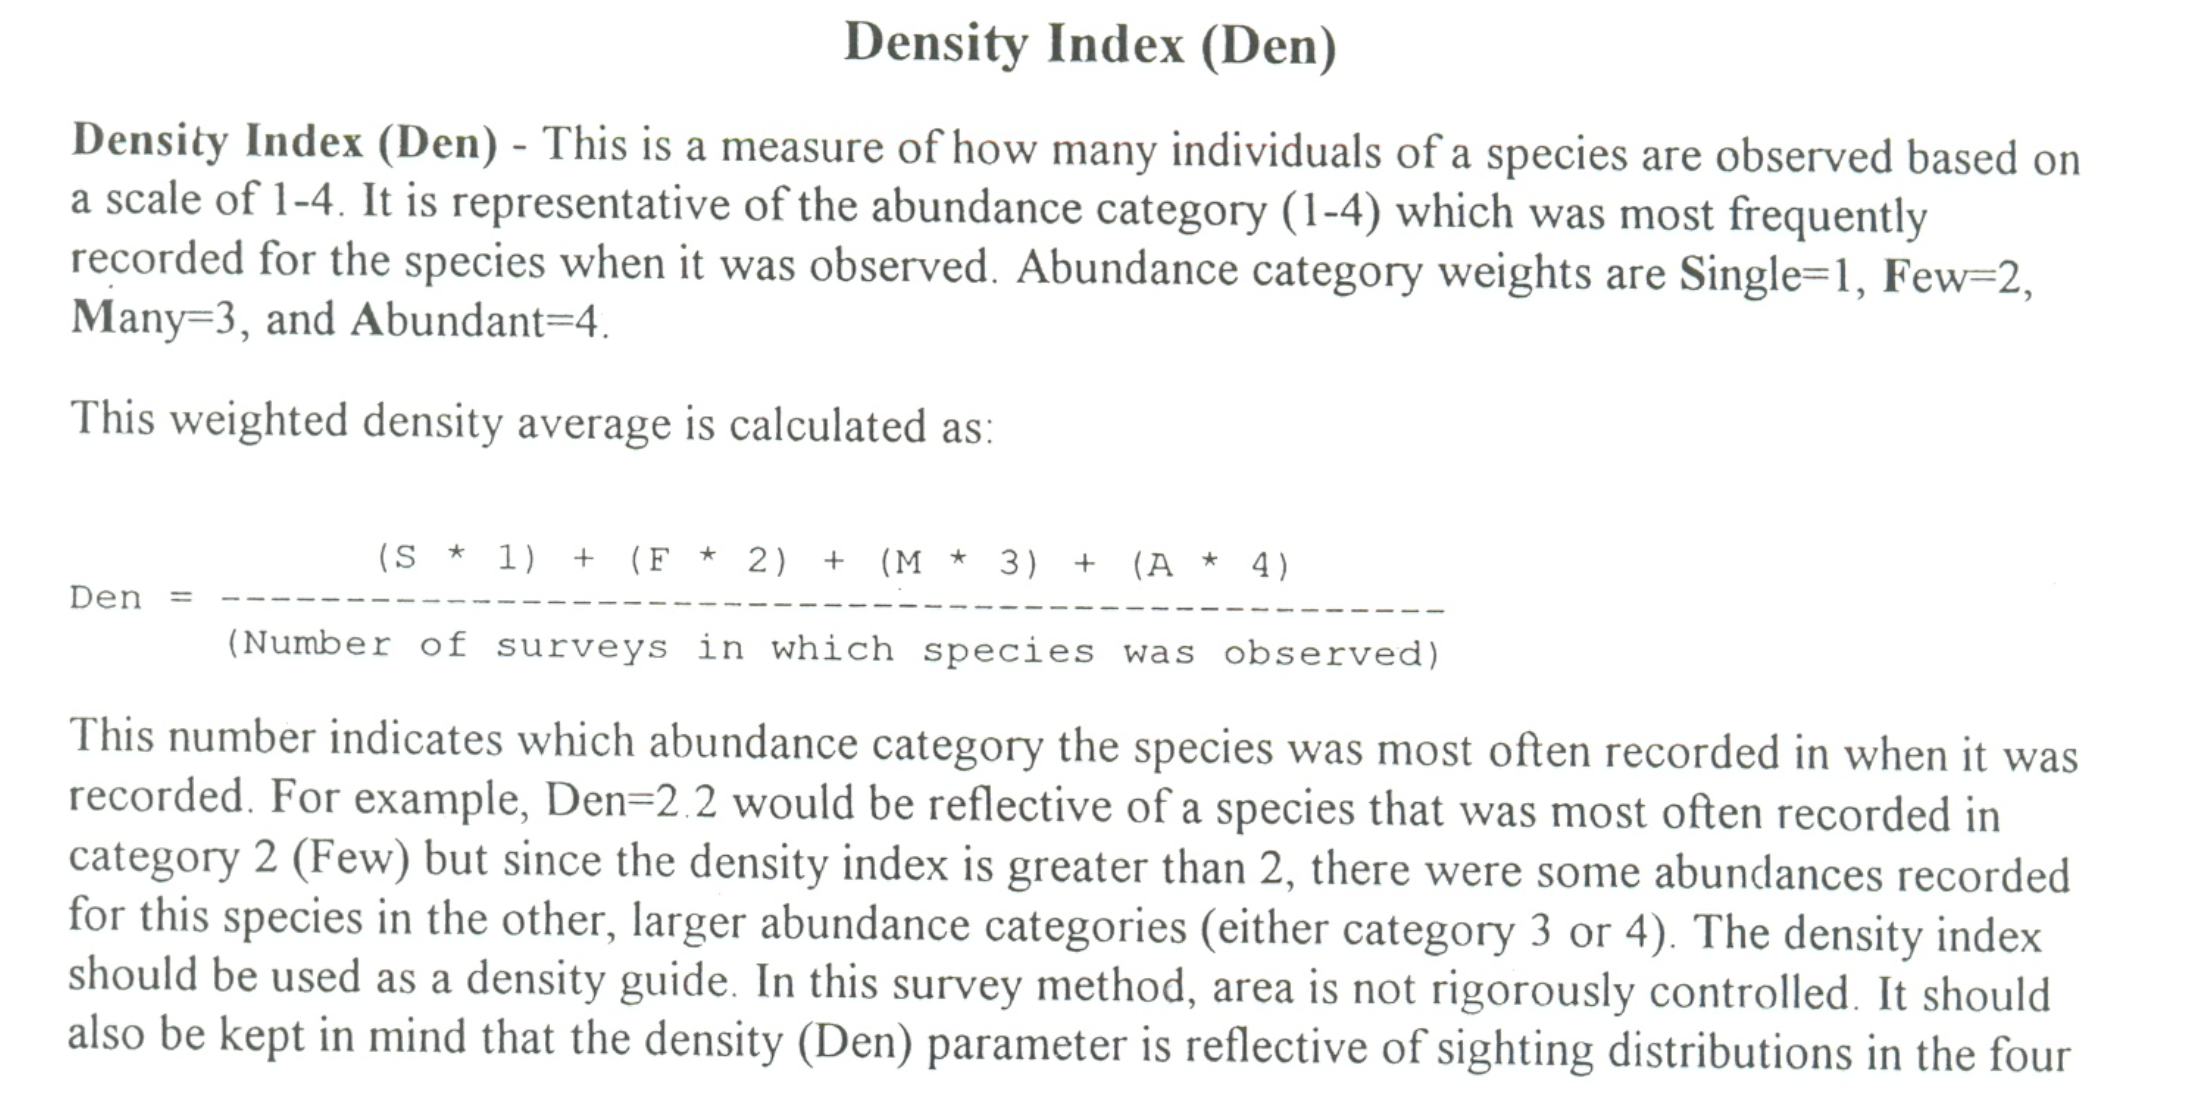
\includegraphics{~/Desktop/IS_CAPSTONE/DEN_STANDARDS.png} As I proceed,
I will perform a statistical analysis, using methods like the T-Test, to
describe important details about similarities and difference in
DENSITY\_INDEX for these fish species. Additionally, I will use linear
mixed effect models, since the data is recorded longitudinally, to
investigate both how species density has changed within each dive site
and how species density has changed between the dive sites. Finally, I
will build a machine learning model to best predict a fish species based
on OOBE/RMSE comparison metrics. This will allow future researchers to
understand under what conditions they may expect to find a certain reef
species. Collectively, these results will help explain the ecology of
coral reef fish species on Grand Cayman Island.

\hypertarget{initial-data-wrangling}{%
\subsection{Initial Data Wrangling}\label{initial-data-wrangling}}

Initially, data consisted of 246 rows and 95 columns. However, the data
set was not in tidy form as information on one variable, Density Index,
was spread across many columns. These columns were also labeled by year
and location, which meant they needed to be separated into individual
variables. To tidy the data, I used the concepts of pivoting and
separating. First, I made the Density Index variable (DENSITY\_INDEX)
using the \texttt{pivot\_longer} function. This function condensed the
columns into one hence making the data set ``longer''. Next, I used the
\texttt{seperate} function to make individual variable columns for the
location and year each observation was collected. Finally, YEAR was
coded as a character variable and I changed it to numeric. After this,
the data set consisted of 22,632 rows and 5 columns. However, some of
the Density Index values followed an outdated version of the REEF scale.
So, values greater than the 4.0 threshold were removed.

\begin{verbatim}
## # A tibble: 6 x 6
##   SPECIES_NAME   FISH_ID  YEAR LOCATION DENSITY_INDEX DEPTH  
##   <chr>            <dbl> <dbl> <chr>            <dbl> <chr>  
## 1 Blue Angelfish       1  1998 CH                   0 Shallow
## 2 Blue Angelfish       1  1998 DG                   2 Deep   
## 3 Blue Angelfish       1  1998 SB                   0 Deep   
## 4 Blue Angelfish       1  1998 SC                   0 Deep   
## 5 Blue Angelfish       1  1998 TF                   0 Deep   
## 6 Blue Angelfish       1  2000 CP                   0 Deep
\end{verbatim}

The \texttt{head} function shows that the five variables consist of two
character variables in SPECIES\_NAME and LOCATION, and three numeric
variables in FISH\_ID, YEAR, and DENSITY\_INDEX. Overall, 12 locations
were studied throughout the duration of data collection. These sites
include, from southeast clockwise to northeast, Bodden Bay Lagoon (BL),
Beach Bay (BB), Smith's Cove (SC), Sunset House (SH), Sea View (SV),
Casuarina Point (CP), Devil's Grotto (DG), Eden's Rock (ER), Cemetery
Reef (CR), Turtle Farm (TF), Spanish Bay (SB), and Mangroves (MG). A
majority of these sites were described and shown geographically in 2018
by Alec Timpe, a Marine Term student of Professor De Stasio. His dive
site image and site description paper can be seen below.
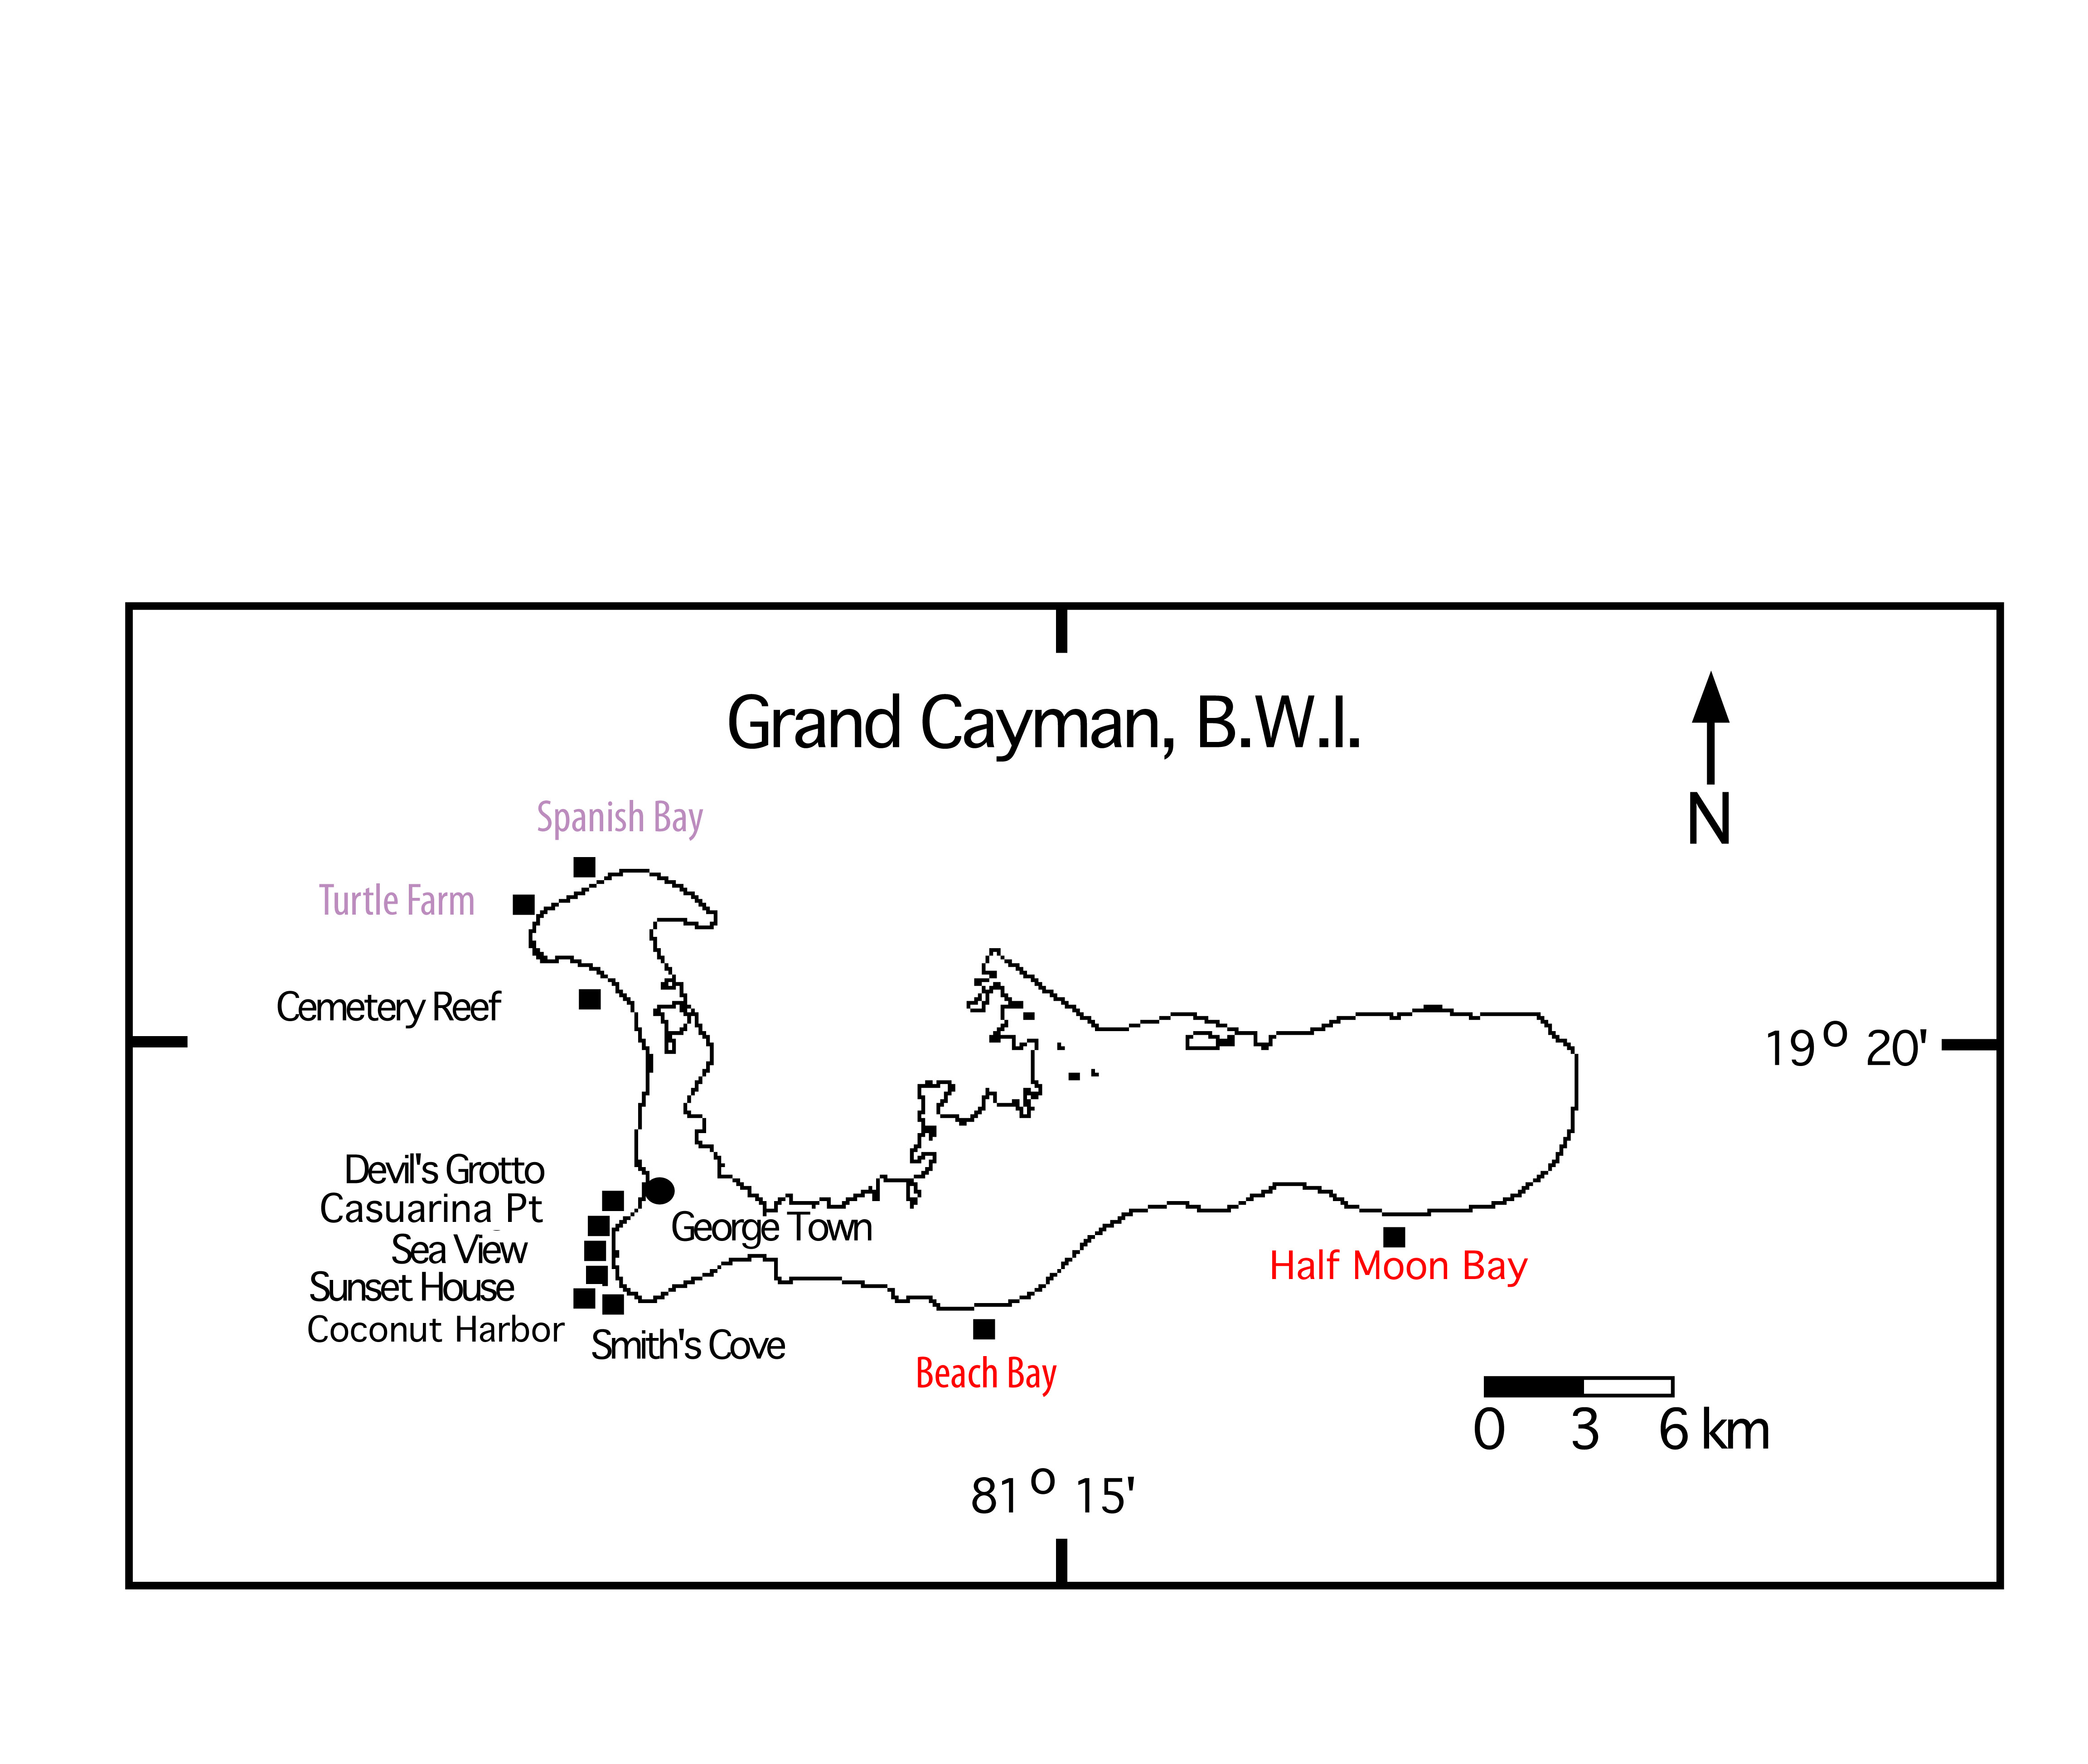
\includegraphics{~/Desktop/IS_CAPSTONE/CAYMAN_MAP.png}

Right click to copy the link, then paste into a web browser:
\href{file:///Users/adam.bruce/Desktop/IS_CAPSTONE/TIMPE_DESCRIPTION.pdf}{Timpe\_Description}

\hypertarget{exploratory-analysis}{%
\subsection{Exploratory Analysis}\label{exploratory-analysis}}

\begin{verbatim}
## # A tibble: 6 x 3
##   SPECIES_NAME          MEAN_DEN STD_DENSITY
##   <chr>                    <dbl>       <dbl>
## 1 Fairy Basslet             2.67       0.437
## 2 Blue Tang                 1.83       1.30 
## 3 Threespot Damselfish      1.82       0.804
## 4 Rock Beauty               1.79       0.532
## 5 Spotfin Butterflyfish     1.71       0.755
## 6 Blue Chromis              1.69       1.70
\end{verbatim}

\begin{table}

\caption{\label{tab:unnamed-chunk-3}Top Six Average Density Index Scores Across All Dive Sites and Years}
\centering
\begin{tabular}[t]{lrr}
\toprule
Species Name & Mean Density & Variance\\
\midrule
Fairy Basslet & 2.672946 & 0.4366565\\
Blue Tang & 1.825481 & 1.2962784\\
Threespot Damselfish & 1.818636 & 0.8040828\\
Rock Beauty & 1.788302 & 0.5317684\\
Spotfin Butterflyfish & 1.714757 & 0.7551484\\
\addlinespace
Blue Chromis & 1.693575 & 1.7015532\\
\bottomrule
\end{tabular}
\end{table}

\begin{table}

\caption{\label{tab:unnamed-chunk-4}Lowest Six Average Density Index Scores Across All Dive Sites and Years for Fish With at least One Sighting (>0)}
\centering
\begin{tabular}[t]{lrr}
\toprule
Species Name & Mean Density & Variance\\
\midrule
Belted Sandfish & 0 & 0\\
Black Jack & 0 & 0\\
Creole-fish & 0 & 0\\
Mottled Mojarra & 0 & 0\\
Orangesided Goby & 0 & 0\\
\addlinespace
Palometa & 0 & 0\\
\bottomrule
\end{tabular}
\end{table}

\begin{figure}
\centering
\includegraphics{BRUCEA_IS_PROJECT_files/figure-latex/unnamed-chunk-5-1.pdf}
\caption{REEF Fish Density Index at Twelve Sampling Locations on Grand
Cayman Island}
\end{figure}

\begin{figure}
\centering
\includegraphics{BRUCEA_IS_PROJECT_files/figure-latex/unnamed-chunk-6-1.pdf}
\caption{Biyearly Mean REEF Fish Density Index Scores on Grand Cayman
Island}
\end{figure}

\includegraphics{BRUCEA_IS_PROJECT_files/figure-latex/unnamed-chunk-7-1.pdf}

\begin{verbatim}
## # A tibble: 22,543 x 6
##    SPECIES_NAME   FISH_ID LOCATION DENSITY_INDEX DEPTH   YEAR1998
##    <chr>            <dbl> <chr>            <dbl> <chr>      <dbl>
##  1 Blue Angelfish       1 CH                   0 Shallow        0
##  2 Blue Angelfish       1 DG                   2 Deep           0
##  3 Blue Angelfish       1 SB                   0 Deep           0
##  4 Blue Angelfish       1 SC                   0 Deep           0
##  5 Blue Angelfish       1 TF                   0 Deep           0
##  6 Blue Angelfish       1 CP                   0 Deep           2
##  7 Blue Angelfish       1 DG                   0 Deep           2
##  8 Blue Angelfish       1 SC                   0 Deep           2
##  9 Blue Angelfish       1 CH                   0 Shallow        2
## 10 Blue Angelfish       1 SB                   0 Deep           2
## # ... with 22,533 more rows
\end{verbatim}

\includegraphics{BRUCEA_IS_PROJECT_files/figure-latex/unnamed-chunk-8-1.pdf}

\includegraphics{BRUCEA_IS_PROJECT_files/figure-latex/unnamed-chunk-9-1.pdf}

\begin{verbatim}
## # A tibble: 6 x 4
##   SPECIES_NAME          MEAN_DI SD_SPECIES     N
##   <chr>                   <dbl>      <dbl> <int>
## 1 Fairy Basslet            2.67      0.437    90
## 2 Blue Tang                1.83      1.30     90
## 3 Threespot Damselfish     1.82      0.804    91
## 4 Rock Beauty              1.79      0.532    92
## 5 Spotfin Butterflyfish    1.71      0.755    91
## 6 Blue Chromis             1.69      1.70     91
\end{verbatim}

\begin{table}

\caption{\label{tab:unnamed-chunk-10}Top Six Mean Density Index Values for Fish Species on Grand Cayman Island}
\centering
\begin{tabu} to \linewidth {>{\raggedright}X>{\raggedleft}X>{\raggedleft}X>{\raggedleft}X}
\toprule
Species Name & Mean Density Index & Standard Deviation & Sample Size\\
\midrule
Fairy Basslet & 2.672946 & 0.4366565 & 90\\
Blue Tang & 1.825481 & 1.2962784 & 90\\
Threespot Damselfish & 1.818636 & 0.8040828 & 91\\
Rock Beauty & 1.788302 & 0.5317684 & 92\\
Spotfin Butterflyfish & 1.714757 & 0.7551484 & 91\\
\addlinespace
Blue Chromis & 1.693575 & 1.7015532 & 91\\
\bottomrule
\end{tabu}
\end{table}

\includegraphics{BRUCEA_IS_PROJECT_files/figure-latex/unnamed-chunk-11-1.pdf}

\includegraphics{BRUCEA_IS_PROJECT_files/figure-latex/unnamed-chunk-12-1.pdf}

\includegraphics{BRUCEA_IS_PROJECT_files/figure-latex/unnamed-chunk-13-1.pdf}

\begin{verbatim}
## # A tibble: 6 x 2
##   SPECIES_NAME           MEAN
##   <chr>                 <dbl>
## 1 Fairy Basslet          2.67
## 2 Blue Tang              1.83
## 3 Threespot Damselfish   1.82
## 4 Rock Beauty            1.79
## 5 Spotfin Butterflyfish  1.71
## 6 Blue Chromis           1.69
\end{verbatim}

\begin{verbatim}
## # A tibble: 15 x 2
##    SPECIES_NAME         MEAN
##    <chr>               <dbl>
##  1 Belted Sandfish         0
##  2 Black Jack              0
##  3 Creole-fish             0
##  4 Mottled Mojarra         0
##  5 Orangesided Goby        0
##  6 Palometa                0
##  7 Peppermint Bass         0
##  8 Reef Croaker            0
##  9 Roughhead Blenny        0
## 10 Round Scad              0
## 11 Sand Perch              0
## 12 Sheepshead              0
## 13 Silver Porgy            0
## 14 Spiny Blenny            0
## 15 Sponge Cardinalfish     0
\end{verbatim}

\includegraphics{BRUCEA_IS_PROJECT_files/figure-latex/unnamed-chunk-14-1.pdf}
\includegraphics{BRUCEA_IS_PROJECT_files/figure-latex/unnamed-chunk-14-2.pdf}

To Do

\hypertarget{mixture-model-probabilistic-model-of-subpopulations-within-an-overall-population.}{%
\section{MIXTURE MODEL PROBABILISTIC MODEL OF SUBPOPULATIONS WITHIN AN
OVERALL
POPULATION.}\label{mixture-model-probabilistic-model-of-subpopulations-within-an-overall-population.}}

\hypertarget{mclus-package-nothing-to-do-with-the-biological-aspect-just-based-on-abundance.}{%
\section{MCLUS Package: Nothing to do with the Biological aspect just
based on
abundance.}\label{mclus-package-nothing-to-do-with-the-biological-aspect-just-based-on-abundance.}}

\hypertarget{two-part}{%
\section{Two Part}\label{two-part}}

\href{https://statistics.laerd.com/spss-tutorials/kruskal-wallis-h-test-using-spss-statistics.php}{KRUSKAL}

\hypertarget{statistical-analysis-on-entire-dataset}{%
\subsubsection{Statistical Analysis on Entire
Dataset}\label{statistical-analysis-on-entire-dataset}}

\begin{verbatim}
## [1] 1.747203
\end{verbatim}

\begin{verbatim}
## [1] 1.715242
\end{verbatim}

\begin{verbatim}
##    
##               BB           CH           CP           CR           DG
##   0 0.0653642065 0.0390738061 0.0897250362 0.0610226725 0.0979257115
##   1 0.0036179450 0.0036179450 0.0084418717 0.0050651230 0.0089242644
##   2 0.0028943560 0.0014471780 0.0077182827 0.0079594790 0.0108538350
##   3 0.0009647853 0.0007235890 0.0024119633 0.0016883743 0.0021707670
##    
##               ER           HM           SB           SC           SH
##   0 0.0246020260 0.0180897250 0.0909310178 0.1025084419 0.0658465991
##   1 0.0031355523 0.0012059817 0.0065123010 0.0074770863 0.0045827303
##   2 0.0024119633 0.0016883743 0.0110950314 0.0079594790 0.0055475157
##   3 0.0004823927 0.0004823927 0.0028943560 0.0026531597 0.0021707670
##    
##               SV           TF
##   0 0.0906898215 0.0851423058
##   1 0.0084418717 0.0062711047
##   2 0.0103714424 0.0106126387
##   3 0.0026531597 0.0019295707
\end{verbatim}

\begin{verbatim}
## 
##  Pearson's Chi-squared test
## 
## data:  Compare_Locations
## X-squared = 35.731, df = 33, p-value = 0.3413
\end{verbatim}

\begin{verbatim}
## # A tibble: 12 x 7
##    LOCATION  MEAN ST.DEV ST.ERR     N upper.95 lower.95
##    <chr>    <dbl>  <dbl>  <dbl> <int>    <dbl>    <dbl>
##  1 BB       0.411  0.840 0.0203  1718    0.451    0.372
##  2 CH       0.379  0.828 0.0265   979    0.431    0.327
##  3 CP       0.443  0.859 0.0173  2454    0.477    0.409
##  4 CR       0.499  0.883 0.0213  1719    0.541    0.458
##  5 DG       0.462  0.886 0.0170  2701    0.496    0.429
##  6 ER       0.520  0.923 0.0341   733    0.587    0.453
##  7 HM       0.402  0.826 0.0373   491    0.475    0.329
##  8 SB       0.446  0.868 0.0176  2429    0.480    0.411
##  9 SC       0.342  0.773 0.0149  2698    0.371    0.313
## 10 SH       0.424  0.851 0.0205  1716    0.464    0.384
## 11 SV       0.483  0.888 0.0179  2453    0.518    0.448
## 12 TF       0.486  0.894 0.0180  2452    0.522    0.451
\end{verbatim}

\includegraphics{BRUCEA_IS_PROJECT_files/figure-latex/unnamed-chunk-15-1.pdf}
\includegraphics{BRUCEA_IS_PROJECT_files/figure-latex/unnamed-chunk-15-2.pdf}
\includegraphics{BRUCEA_IS_PROJECT_files/figure-latex/unnamed-chunk-15-3.pdf}
\includegraphics{BRUCEA_IS_PROJECT_files/figure-latex/unnamed-chunk-15-4.pdf}
\includegraphics{BRUCEA_IS_PROJECT_files/figure-latex/unnamed-chunk-15-5.pdf}

\begin{verbatim}
## Levene's Test for Homogeneity of Variance (center = median)
##          Df F value    Pr(>F)    
## group    11  6.6317 3.504e-11 ***
##       22531                      
## ---
## Signif. codes:  0 '***' 0.001 '**' 0.01 '*' 0.05 '.' 0.1 ' ' 1
\end{verbatim}

\begin{verbatim}
## 
##  Shapiro-Wilk normality test
## 
## data:  CAYMAN_SUBSET
## W = 0.56506, p-value < 2.2e-16
\end{verbatim}

\begin{verbatim}
## # A tibble: 22,543 x 6
##    SPECIES_NAME   FISH_ID  YEAR LOCATION DENSITY_INDEX DEPTH  
##    <chr>            <dbl> <dbl> <chr>            <dbl> <chr>  
##  1 Blue Angelfish       1  1998 CH                0    Shallow
##  2 Blue Angelfish       1  1998 DG                1.10 Deep   
##  3 Blue Angelfish       1  1998 SB                0    Deep   
##  4 Blue Angelfish       1  1998 SC                0    Deep   
##  5 Blue Angelfish       1  1998 TF                0    Deep   
##  6 Blue Angelfish       1  2000 CP                0    Deep   
##  7 Blue Angelfish       1  2000 DG                0    Deep   
##  8 Blue Angelfish       1  2000 SC                0    Deep   
##  9 Blue Angelfish       1  2000 CH                0    Shallow
## 10 Blue Angelfish       1  2000 SB                0    Deep   
## # ... with 22,533 more rows
\end{verbatim}

\begin{verbatim}
## Levene's Test for Homogeneity of Variance (center = median)
##          Df F value    Pr(>F)    
## group    11  7.2889 1.442e-12 ***
##       22531                      
## ---
## Signif. codes:  0 '***' 0.001 '**' 0.01 '*' 0.05 '.' 0.1 ' ' 1
\end{verbatim}

\begin{verbatim}
## 
##  Shapiro-Wilk normality test
## 
## data:  CAYMAN_LOG_SUBSET
## W = 0.57299, p-value < 2.2e-16
\end{verbatim}

\includegraphics{BRUCEA_IS_PROJECT_files/figure-latex/unnamed-chunk-15-6.pdf}
\includegraphics{BRUCEA_IS_PROJECT_files/figure-latex/unnamed-chunk-15-7.pdf}
\includegraphics{BRUCEA_IS_PROJECT_files/figure-latex/unnamed-chunk-15-8.pdf}
\includegraphics{BRUCEA_IS_PROJECT_files/figure-latex/unnamed-chunk-15-9.pdf}
\includegraphics{BRUCEA_IS_PROJECT_files/figure-latex/unnamed-chunk-15-10.pdf}

\begin{verbatim}
## Levene's Test for Homogeneity of Variance (center = median)
##          Df F value    Pr(>F)    
## group    11  6.6317 3.504e-11 ***
##       22531                      
## ---
## Signif. codes:  0 '***' 0.001 '**' 0.01 '*' 0.05 '.' 0.1 ' ' 1
\end{verbatim}

\begin{verbatim}
## 
##  Shapiro-Wilk normality test
## 
## data:  CAYMAN_SQRT_SUBSET
## W = 0.56607, p-value < 2.2e-16
\end{verbatim}

\includegraphics{BRUCEA_IS_PROJECT_files/figure-latex/unnamed-chunk-15-11.pdf}
\includegraphics{BRUCEA_IS_PROJECT_files/figure-latex/unnamed-chunk-15-12.pdf}
\includegraphics{BRUCEA_IS_PROJECT_files/figure-latex/unnamed-chunk-15-13.pdf}
\includegraphics{BRUCEA_IS_PROJECT_files/figure-latex/unnamed-chunk-15-14.pdf}
\includegraphics{BRUCEA_IS_PROJECT_files/figure-latex/unnamed-chunk-15-15.pdf}
\includegraphics{BRUCEA_IS_PROJECT_files/figure-latex/unnamed-chunk-15-16.pdf}

\begin{verbatim}
## 
##  Kruskal-Wallis rank sum test
## 
## data:  DENSITY_INDEX by LOCATION
## Kruskal-Wallis chi-squared = 84.794, df = 11, p-value = 1.733e-13
\end{verbatim}

\includegraphics{BRUCEA_IS_PROJECT_files/figure-latex/unnamed-chunk-15-17.pdf}

\hypertarget{grouping-fish-by-family}{%
\subsubsection{GROUPING FISH BY FAMILY}\label{grouping-fish-by-family}}

\hypertarget{stats-on-new-family-variable}{%
\subsubsection{Stats On New Family
Variable}\label{stats-on-new-family-variable}}

\begin{verbatim}
##     
##        Apogonidae   Carangidae     Gobiidae   Haemulidae Holocentridae
##   BB 0.0018631061 0.0037262121 0.0055893182 0.0049682828  0.0018631061
##   CH 0.0010646320 0.0021292641 0.0031495364 0.0028390188  0.0010646320
##   CP 0.0026615801 0.0053231602 0.0079403806 0.0070975469  0.0026615801
##   CR 0.0018631061 0.0037262121 0.0055893182 0.0049682828  0.0018631061
##   DG 0.0029277381 0.0058554762 0.0087832143 0.0078073016  0.0028833784
##   ER 0.0007984740 0.0015969481 0.0023510624 0.0021292641  0.0007541144
##   HM 0.0005323160 0.0010646320 0.0015525884 0.0014195094  0.0005323160
##   SB 0.0026615801 0.0052788005 0.0079847403 0.0070531872  0.0025285011
##   SC 0.0029277381 0.0058554762 0.0087832143 0.0078073016  0.0028833784
##   SH 0.0018631061 0.0037262121 0.0055893182 0.0049682828  0.0018187464
##   SV 0.0026615801 0.0053231602 0.0079847403 0.0070088276  0.0026615801
##   TF 0.0026615801 0.0053231602 0.0079403806 0.0070975469  0.0026615801
##     
##          Labridae   Lutjanidae        Other Pomacentridae     Scaridae
##   BB 0.0046577652 0.0031051768 0.0306525307  0.0042585281 0.0040367298
##   CH 0.0026615801 0.0017743867 0.0174777093  0.0023954221 0.0023067027
##   CP 0.0066095906 0.0044359668 0.0438273522  0.0061659939 0.0057223972
##   CR 0.0046577652 0.0031051768 0.0306525307  0.0043028878 0.0040367298
##   DG 0.0072749856 0.0048795635 0.0482633190  0.0067426696 0.0063434326
##   ER 0.0019961851 0.0013307900 0.0130417424  0.0018631061 0.0017300271
##   HM 0.0013307900 0.0008871934 0.0087832143  0.0012420707 0.0011533514
##   SB 0.0065652309 0.0043028878 0.0434724748  0.0059441955 0.0056336779
##   SC 0.0072306259 0.0048795635 0.0481745997  0.0067426696 0.0063434326
##   SH 0.0046577652 0.0030608171 0.0306081711  0.0043028878 0.0040367298
##   SV 0.0066539502 0.0044359668 0.0437386328  0.0061659939 0.0057667569
##   TF 0.0066539502 0.0044359668 0.0437386328  0.0060772745 0.0057667569
##     
##        Serranidae     Sparidae
##   BB 0.0093155303 0.0021736237
##   CH 0.0053231602 0.0012420707
##   CP 0.0133079005 0.0031051768
##   CR 0.0093155303 0.0021736237
##   DG 0.0146386905 0.0034156945
##   ER 0.0039923701 0.0009315530
##   HM 0.0026615801 0.0006210354
##   SB 0.0132191811 0.0031051768
##   SC 0.0146386905 0.0034156945
##   SH 0.0093155303 0.0021736237
##   SV 0.0133079005 0.0031051768
##   TF 0.0133079005 0.0031051768
\end{verbatim}

\begin{verbatim}
## # A tibble: 12 x 7
##    SCIENTIFIC_FAMILY  MEAN ST.DEV  ST.ERR     N upper.95 lower.95
##    <chr>             <dbl>  <dbl>   <dbl> <int>    <dbl>    <dbl>
##  1 Apogonidae        0.205  0.628 0.0267    552    0.258    0.153
##  2 Carangidae        0.181  0.594 0.0179   1103    0.216    0.146
##  3 Gobiidae          0.178  0.608 0.0150   1651    0.207    0.149
##  4 Haemulidae        0.322  0.767 0.0200   1469    0.361    0.283
##  5 Holocentridae     1.14   1.17  0.0500    545    1.23     1.04 
##  6 Labridae          0.470  0.860 0.0232   1374    0.515    0.424
##  7 Lutjanidae        0.568  0.904 0.0299    916    0.627    0.510
##  8 Other             0.417  0.816 0.00857  9072    0.434    0.400
##  9 Pomacentridae     1.17   1.27  0.0356   1267    1.24     1.10 
## 10 Scaridae          0.706  1.02  0.0295   1192    0.763    0.648
## 11 Serranidae        0.299  0.648 0.0123   2758    0.323    0.275
## 12 Sparidae          0.247  0.706 0.0278    644    0.302    0.193
\end{verbatim}

\includegraphics{BRUCEA_IS_PROJECT_files/figure-latex/unnamed-chunk-17-1.pdf}

\begin{verbatim}
## Levene's Test for Homogeneity of Variance (center = median)
##          Df F value    Pr(>F)    
## group    11  188.13 < 2.2e-16 ***
##       22531                      
## ---
## Signif. codes:  0 '***' 0.001 '**' 0.01 '*' 0.05 '.' 0.1 ' ' 1
\end{verbatim}

\includegraphics{BRUCEA_IS_PROJECT_files/figure-latex/unnamed-chunk-17-2.pdf}

\begin{verbatim}
## 
##  Kruskal-Wallis rank sum test
## 
## data:  DENSITY_INDEX by SCIENTIFIC_FAMILY
## Kruskal-Wallis chi-squared = 1553.1, df = 11, p-value < 2.2e-16
\end{verbatim}

\includegraphics{BRUCEA_IS_PROJECT_files/figure-latex/unnamed-chunk-17-3.pdf}
\#\#\# Graphical Visualization by Families

\begin{table}

\caption{\label{tab:unnamed-chunk-18}Summary Statistics for Twelve Families of Fish on Grand Cayman Island}
\centering
\begin{tabu} to \linewidth {>{\raggedright}X>{\raggedleft}X>{\raggedleft}X>{\raggedleft}X>{\raggedleft}X>{\raggedleft}X>{\raggedleft}X}
\toprule
Scientific Family & Mean Density Index & Standard Deviation & Standard Error & Sample Size & Upper 95\% CI & Lower 95\% CI\\
\midrule
Pomacentridae & 1.1735051 & 1.2654297 & 0.0355508 & 1267 & 1.2431834 & 1.1038267\\
Holocentridae & 1.1365635 & 1.1671619 & 0.0499957 & 545 & 1.2345533 & 1.0385737\\
Scaridae & 0.7055519 & 1.0169367 & 0.0294548 & 1192 & 0.7632822 & 0.6478216\\
Lutjanidae & 0.5683379 & 0.9041616 & 0.0298743 & 916 & 0.6268906 & 0.5097853\\
Labridae & 0.4696159 & 0.8600878 & 0.0232033 & 1374 & 0.5150935 & 0.4241383\\
\addlinespace
Other & 0.4168636 & 0.8162553 & 0.0085699 & 9072 & 0.4336602 & 0.4000669\\
Haemulidae & 0.3222590 & 0.7671973 & 0.0200169 & 1469 & 0.3614914 & 0.2830267\\
Serranidae & 0.2990534 & 0.6480974 & 0.0123408 & 2758 & 0.3232409 & 0.2748659\\
Sparidae & 0.2472986 & 0.7055934 & 0.0278043 & 644 & 0.3017940 & 0.1928033\\
Apogonidae & 0.2052027 & 0.6280289 & 0.0267307 & 552 & 0.2575939 & 0.1528115\\
\addlinespace
Carangidae & 0.1812783 & 0.5939445 & 0.0178837 & 1103 & 0.2163298 & 0.1462269\\
Gobiidae & 0.1778428 & 0.6081996 & 0.0149683 & 1651 & 0.2071802 & 0.1485055\\
\bottomrule
\end{tabu}
\end{table}

\includegraphics{BRUCEA_IS_PROJECT_files/figure-latex/unnamed-chunk-19-1.pdf}

\includegraphics{BRUCEA_IS_PROJECT_files/figure-latex/unnamed-chunk-20-1.pdf}

\includegraphics{BRUCEA_IS_PROJECT_files/figure-latex/unnamed-chunk-21-1.pdf}

\hypertarget{modeling}{%
\subsubsection{Modeling}\label{modeling}}

TWO PART MODEL: A Specialized Mixture Model

\href{https://journals.sagepub.com/doi/pdf/10.1177/1536867X1501500102}{TPM}

why?

A two-part model is a flexible statistical model specifically designed
to deal with limited dependent variables. The distinguishing feature of
these variables is that the range of values they may assume has a lower
bound occurring in a fair number of observations.

How?

The zeros are typically handled using a model for the probability of a
positive outcome:

φ(y \textgreater{} 0) = Pr(y \textgreater{} 0\textbar x) = F(xδ)

where x is a vector of explanatory variables, δ is the corresponding
vector of parameters to be estimated, and F is the cumulative
distribution function of an independent and identically distributed
error term, typically chosen to be from extreme value (logit) or normal
(probit) distributions

\href{https://www.theanalysisfactor.com/what-is-logit-function/}{LOGIT}

For the positives, the model is usually represented as:

φ(y\textbar y \textgreater{} 0, x) = g(xγ)

where x is a vector of explanatory variables, γ is the corresponding
vector of parameters to be estimated, and g is an appropriate density
function for y\textbar y \textgreater{} 0

TWO PART MODEL OKAY?

\href{https://stats.stackexchange.com/questions/345474/residual-vs-fitted}{DISCRETE\_CONTINUOUS}
\href{https://stats.stackexchange.com/questions/120751/not-sure-about-the-interpretation-of-this-residual-plot}{MORE\_DIS\_CON}

\begin{verbatim}
## # A tibble: 1 x 2
##   NUMBER_ZEROS NUMBER_NONZEROS
##          <int>           <int>
## 1        17230            5313
\end{verbatim}

\includegraphics{BRUCEA_IS_PROJECT_files/figure-latex/unnamed-chunk-22-1.pdf}
\includegraphics{BRUCEA_IS_PROJECT_files/figure-latex/unnamed-chunk-22-2.pdf}

\begin{verbatim}
## # A tibble: 6 x 7
##   SPECIES_NAME   FISH_ID  YEAR LOCATION DENSITY_INDEX DEPTH   SCIENTIFIC_FAMILY
##   <chr>            <dbl> <dbl> <chr>            <dbl> <chr>   <chr>            
## 1 Blue Angelfish       1  1998 CH                   0 Shallow Other            
## 2 Blue Angelfish       1  1998 DG                   1 Deep    Other            
## 3 Blue Angelfish       1  1998 SB                   0 Deep    Other            
## 4 Blue Angelfish       1  1998 SC                   0 Deep    Other            
## 5 Blue Angelfish       1  1998 TF                   0 Deep    Other            
## 6 Blue Angelfish       1  2000 CP                   0 Deep    Other
\end{verbatim}

\begin{verbatim}
##  SPECIES_NAME          FISH_ID           YEAR        LOCATION        
##  Length:22543       Min.   :  1.0   Min.   :1998   Length:22543      
##  Class :character   1st Qu.: 62.0   1st Qu.:2004   Class :character  
##  Mode  :character   Median :124.0   Median :2010   Mode  :character  
##                     Mean   :123.5   Mean   :2009                     
##                     3rd Qu.:185.0   3rd Qu.:2014                     
##                     Max.   :246.0   Max.   :2018                     
##  DENSITY_INDEX       DEPTH           SCIENTIFIC_FAMILY 
##  Min.   :0.0000   Length:22543       Length:22543      
##  1st Qu.:0.0000   Class :character   Class :character  
##  Median :0.0000   Mode  :character   Mode  :character  
##  Mean   :0.2357                                        
##  3rd Qu.:0.0000                                        
##  Max.   :1.0000
\end{verbatim}

\begin{verbatim}
##  SPECIES_NAME          FISH_ID           YEAR        LOCATION        
##  Length:22543       Min.   :  1.0   Min.   :1998   Length:22543      
##  Class :character   1st Qu.: 62.0   1st Qu.:2004   Class :character  
##  Mode  :character   Median :124.0   Median :2010   Mode  :character  
##                     Mean   :123.5   Mean   :2009                     
##                     3rd Qu.:185.0   3rd Qu.:2014                     
##                     Max.   :246.0   Max.   :2018                     
##  DENSITY_INDEX       DEPTH           SCIENTIFIC_FAMILY 
##  Min.   :0.0000   Length:22543       Length:22543      
##  1st Qu.:0.0000   Class :character   Class :character  
##  Median :0.0000   Mode  :character   Mode  :character  
##  Mean   :0.2357                                        
##  3rd Qu.:0.0000                                        
##  Max.   :1.0000
\end{verbatim}

\includegraphics{BRUCEA_IS_PROJECT_files/figure-latex/unnamed-chunk-22-3.pdf}
\includegraphics{BRUCEA_IS_PROJECT_files/figure-latex/unnamed-chunk-22-4.pdf}
\includegraphics{BRUCEA_IS_PROJECT_files/figure-latex/unnamed-chunk-22-5.pdf}
\includegraphics{BRUCEA_IS_PROJECT_files/figure-latex/unnamed-chunk-22-6.pdf}

\begin{verbatim}
## 
## Call:
## lm(formula = DENSITY_INDEX ~ YEAR + LOCATION + SCIENTIFIC_FAMILY, 
##     data = CAYMAN_NO_ZEROS)
## 
## Residuals:
##      Min       1Q   Median       3Q      Max 
## -1.48441 -0.53776  0.02514  0.39531  2.12473 
## 
## Coefficients:
##                                 Estimate Std. Error t value Pr(>|t|)    
## (Intercept)                    18.746855   2.978887   6.293 3.36e-10 ***
## YEAR                           -0.008330   0.001482  -5.619 2.02e-08 ***
## LOCATIONCH                      0.006098   0.056702   0.108  0.91437    
## LOCATIONCP                     -0.050214   0.042300  -1.187  0.23525    
## LOCATIONCR                     -0.068164   0.044375  -1.536  0.12457    
## LOCATIONDG                     -0.005260   0.041457  -0.127  0.89905    
## LOCATIONER                      0.047679   0.056643   0.842  0.39997    
## LOCATIONHM                     -0.041584   0.070504  -0.590  0.55534    
## LOCATIONSB                     -0.008841   0.042516  -0.208  0.83528    
## LOCATIONSC                     -0.078548   0.043704  -1.797  0.07235 .  
## LOCATIONSH                      0.005918   0.046569   0.127  0.89888    
## LOCATIONSV                     -0.018147   0.041701  -0.435  0.66345    
## LOCATIONTF                     -0.009118   0.041709  -0.219  0.82695    
## SCIENTIFIC_FAMILYCarangidae    -0.068427   0.104937  -0.652  0.51438    
## SCIENTIFIC_FAMILYGobiidae       0.100639   0.099986   1.007  0.31421    
## SCIENTIFIC_FAMILYHaemulidae    -0.051533   0.093722  -0.550  0.58245    
## SCIENTIFIC_FAMILYHolocentridae  0.238211   0.092645   2.571  0.01016 *  
## SCIENTIFIC_FAMILYLabridae      -0.205604   0.090808  -2.264  0.02360 *  
## SCIENTIFIC_FAMILYLutjanidae    -0.153563   0.092485  -1.660  0.09689 .  
## SCIENTIFIC_FAMILYOther         -0.229688   0.085542  -2.685  0.00727 ** 
## SCIENTIFIC_FAMILYPomacentridae  0.373821   0.088163   4.240 2.27e-05 ***
## SCIENTIFIC_FAMILYScaridae       0.009882   0.089947   0.110  0.91252    
## SCIENTIFIC_FAMILYSerranidae    -0.461519   0.088767  -5.199 2.08e-07 ***
## SCIENTIFIC_FAMILYSparidae       0.071857   0.111073   0.647  0.51770    
## ---
## Signif. codes:  0 '***' 0.001 '**' 0.01 '*' 0.05 '.' 0.1 ' ' 1
## 
## Residual standard error: 0.6371 on 5289 degrees of freedom
## Multiple R-squared:  0.1293, Adjusted R-squared:  0.1255 
## F-statistic: 34.16 on 23 and 5289 DF,  p-value: < 2.2e-16
\end{verbatim}

Consider Predicting on next few years\ldots{} Time Series Analysis.

\hypertarget{k-means-and-hierarchical-clustering}{%
\subsubsection{K MEANS AND HIERARCHICAL
CLUSTERING}\label{k-means-and-hierarchical-clustering}}

\href{https://www.r-bloggers.com/2016/06/clustering-mixed-data-types-in-r/}{Clustering}

\begin{verbatim}
## 14111328 dissimilarities, summarized :
##    Min. 1st Qu.  Median    Mean 3rd Qu.    Max. 
##  0.0000  0.4692  0.6289  0.6019  0.6692  1.0000 
## Metric :  mixed ;  Types = N, N, I, N, N 
## Number of objects : 5313
\end{verbatim}

\begin{verbatim}
## # A tibble: 2 x 5
##   YEAR  LOCATION DENSITY_INDEX DEPTH SCIENTIFIC_FAMILY
##   <fct> <fct>            <dbl> <fct> <fct>            
## 1 2008  SC                2.9  Deep  Holocentridae    
## 2 2008  SC                2.89 Deep  Holocentridae
\end{verbatim}

\begin{verbatim}
## # A tibble: 2 x 5
##   YEAR  LOCATION DENSITY_INDEX DEPTH   SCIENTIFIC_FAMILY
##   <fct> <fct>            <dbl> <fct>   <fct>            
## 1 2018  SC                3.88 Deep    Pomacentridae    
## 2 1998  CH                1    Shallow Other
\end{verbatim}

\includegraphics{BRUCEA_IS_PROJECT_files/figure-latex/unnamed-chunk-23-1.pdf}

\begin{verbatim}
## [[1]]
##       YEAR        LOCATION   DENSITY_INDEX       DEPTH    
##  2018   :261   DG     :403   Min.   :1.000   Deep   :539  
##  1998   : 65   CR     : 43   1st Qu.:1.667   Shallow:  0  
##  2002   : 50   SV     : 40   Median :2.000                
##  2004   : 37   SH     : 39   Mean   :1.967                
##  2000   : 34   CP     : 14   3rd Qu.:2.183                
##  2006   : 34   BB     :  0   Max.   :3.500                
##  (Other): 58   (Other):  0                                
##      SCIENTIFIC_FAMILY    cluster 
##  Other        :262     Min.   :1  
##  Scaridae     : 48     1st Qu.:1  
##  Serranidae   : 38     Median :1  
##  Lutjanidae   : 32     Mean   :1  
##  Haemulidae   : 29     3rd Qu.:1  
##  Holocentridae: 29     Max.   :1  
##  (Other)      :101                
## 
## [[2]]
##       YEAR        LOCATION   DENSITY_INDEX       DEPTH    
##  2012   :319   SV     :386   Min.   :1.000   Deep   :641  
##  2002   : 76   SH     : 65   1st Qu.:1.000   Shallow:  0  
##  2000   : 41   CP     : 52   Median :1.667                
##  2010   : 39   TF     : 46   Mean   :1.745                
##  2006   : 38   CR     : 23   3rd Qu.:2.000                
##  2004   : 35   BB     : 20   Max.   :3.500                
##  (Other): 93   (Other): 49                                
##      SCIENTIFIC_FAMILY    cluster 
##  Other        :353     Min.   :2  
##  Labridae     : 45     1st Qu.:2  
##  Lutjanidae   : 42     Median :2  
##  Scaridae     : 42     Mean   :2  
##  Holocentridae: 36     3rd Qu.:2  
##  Pomacentridae: 33     Max.   :2  
##  (Other)      : 90                
## 
## [[3]]
##       YEAR        LOCATION   DENSITY_INDEX       DEPTH    
##  2008   :292   SC     :378   Min.   :1.000   Deep   :671  
##  2010   : 66   CP     : 59   1st Qu.:1.600   Shallow:  0  
##  2006   : 58   CR     : 49   Median :2.000                
##  2002   : 47   SH     : 48   Mean   :1.930                
##  2000   : 43   DG     : 40   3rd Qu.:2.200                
##  2014   : 43   BB     : 37   Max.   :3.667                
##  (Other):122   (Other): 60                                
##      SCIENTIFIC_FAMILY    cluster 
##  Other        :346     Min.   :3  
##  Labridae     : 51     1st Qu.:3  
##  Scaridae     : 47     Median :3  
##  Pomacentridae: 39     Mean   :3  
##  Holocentridae: 38     3rd Qu.:3  
##  Haemulidae   : 33     Max.   :3  
##  (Other)      :117                
## 
## [[4]]
##       YEAR        LOCATION   DENSITY_INDEX       DEPTH    
##  2014   :333   BB     :233   Min.   :1.000   Deep   :507  
##  2002   : 47   SH     : 51   1st Qu.:1.800   Shallow:  0  
##  2004   : 37   CP     : 49   Median :2.000                
##  2018   : 34   TF     : 47   Mean   :2.011                
##  2012   : 33   CR     : 45   3rd Qu.:2.333                
##  2000   : 23   DG     : 45   Max.   :3.857                
##  (Other):  0   (Other): 37                                
##      SCIENTIFIC_FAMILY    cluster 
##  Other        :228     Min.   :4  
##  Scaridae     : 66     1st Qu.:4  
##  Pomacentridae: 42     Median :4  
##  Labridae     : 37     Mean   :4  
##  Lutjanidae   : 29     3rd Qu.:4  
##  Holocentridae: 26     Max.   :4  
##  (Other)      : 79                
## 
## [[5]]
##       YEAR        LOCATION   DENSITY_INDEX       DEPTH      SCIENTIFIC_FAMILY
##  2018   :330   TF     :407   Min.   :1.000   Deep   :652   Other     :394    
##  2000   : 53   CP     : 58   1st Qu.:1.000   Shallow:  0   Scaridae  : 54    
##  2006   : 51   SH     : 45   Median :1.250                 Serranidae: 43    
##  1998   : 49   SC     : 41   Mean   :1.475                 Labridae  : 36    
##  2002   : 45   SB     : 37   3rd Qu.:2.000                 Lutjanidae: 29    
##  2016   : 41   CR     : 31   Max.   :3.500                 Haemulidae: 23    
##  (Other): 83   (Other): 33                                 (Other)   : 73    
##     cluster 
##  Min.   :5  
##  1st Qu.:5  
##  Median :5  
##  Mean   :5  
##  3rd Qu.:5  
##  Max.   :5  
##             
## 
## [[6]]
##       YEAR        LOCATION   DENSITY_INDEX       DEPTH    
##  2010   :429   SB     :433   Min.   :1.000   Deep   :727  
##  2014   : 63   DG     : 70   1st Qu.:1.500   Shallow: 63  
##  1998   : 53   HM     : 63   Median :2.000                
##  2006   : 53   CR     : 61   Mean   :1.934                
##  2018   : 44   SH     : 52   3rd Qu.:2.200                
##  2000   : 42   CP     : 43   Max.   :3.667                
##  (Other):106   (Other): 68                                
##      SCIENTIFIC_FAMILY    cluster 
##  Other        :361     Min.   :6  
##  Labridae     : 59     1st Qu.:6  
##  Holocentridae: 55     Median :6  
##  Pomacentridae: 55     Mean   :6  
##  Scaridae     : 53     3rd Qu.:6  
##  Lutjanidae   : 49     Max.   :6  
##  (Other)      :158                
## 
## [[7]]
##       YEAR        LOCATION   DENSITY_INDEX       DEPTH    
##  2018   :108   ER     :198   Min.   :1.000   Deep   :  0  
##  2012   : 61   BB     :  0   1st Qu.:1.271   Shallow:198  
##  2016   : 29   CH     :  0   Median :2.000                
##  1998   :  0   CP     :  0   Mean   :1.915                
##  2000   :  0   CR     :  0   3rd Qu.:2.333                
##  2002   :  0   DG     :  0   Max.   :3.667                
##  (Other):  0   (Other):  0                                
##      SCIENTIFIC_FAMILY    cluster 
##  Other        :82      Min.   :7  
##  Pomacentridae:25      1st Qu.:7  
##  Scaridae     :17      Median :7  
##  Serranidae   :17      Mean   :7  
##  Holocentridae:12      3rd Qu.:7  
##  Labridae     :12      Max.   :7  
##  (Other)      :33                 
## 
## [[8]]
##       YEAR       LOCATION   DENSITY_INDEX       DEPTH         SCIENTIFIC_FAMILY
##  2014   :77   CH     :193   Min.   :1.000   Deep   :  0   Other        :89     
##  1998   :49   HM     : 31   1st Qu.:1.333   Shallow:224   Pomacentridae:30     
##  2000   :37   BB     :  0   Median :2.000                 Serranidae   :26     
##  2004   :31   CP     :  0   Mean   :1.939                 Scaridae     :18     
##  2016   :30   CR     :  0   3rd Qu.:2.425                 Labridae     :17     
##  2002   : 0   DG     :  0   Max.   :3.889                 Lutjanidae   :13     
##  (Other): 0   (Other):  0                                 (Other)      :31     
##     cluster 
##  Min.   :8  
##  1st Qu.:8  
##  Median :8  
##  Mean   :8  
##  3rd Qu.:8  
##  Max.   :8  
##             
## 
## [[9]]
##       YEAR        LOCATION   DENSITY_INDEX       DEPTH      SCIENTIFIC_FAMILY
##  2012   :176   CR     :183   Min.   :1.000   Deep   :448   Serranidae:273    
##  2010   : 55   CP     : 46   1st Qu.:1.000   Shallow:  9   Labridae  : 41    
##  2006   : 53   SH     : 40   Median :1.000                 Scaridae  : 29    
##  2018   : 44   SB     : 37   Mean   :1.302                 Other     : 26    
##  2014   : 31   DG     : 34   3rd Qu.:1.500                 Haemulidae: 20    
##  2008   : 29   BB     : 32   Max.   :3.286                 Lutjanidae: 20    
##  (Other): 69   (Other): 85                                 (Other)   : 48    
##     cluster 
##  Min.   :9  
##  1st Qu.:9  
##  Median :9  
##  Mean   :9  
##  3rd Qu.:9  
##  Max.   :9  
##             
## 
## [[10]]
##       YEAR        LOCATION   DENSITY_INDEX       DEPTH    
##  2018   :242   CP     :268   Min.   :1.000   Deep   :630  
##  2002   : 54   SV     : 55   1st Qu.:2.000   Shallow:  4  
##  2000   : 53   DG     : 48   Median :2.500                
##  2014   : 46   SB     : 48   Mean   :2.471                
##  2006   : 45   TF     : 47   3rd Qu.:3.000                
##  2012   : 43   SH     : 46   Max.   :3.875                
##  (Other):151   (Other):122                                
##      SCIENTIFIC_FAMILY    cluster  
##  Pomacentridae:362     Min.   :10  
##  Scaridae     : 49     1st Qu.:10  
##  Holocentridae: 37     Median :10  
##  Labridae     : 36     Mean   :10  
##  Haemulidae   : 28     3rd Qu.:10  
##  Lutjanidae   : 27     Max.   :10  
##  (Other)      : 95
\end{verbatim}

\begin{verbatim}
## # A tibble: 10 x 5
##    YEAR  LOCATION DENSITY_INDEX DEPTH   SCIENTIFIC_FAMILY
##    <fct> <fct>            <dbl> <fct>   <fct>            
##  1 2018  DG                2    Deep    Other            
##  2 2012  SV                1.67 Deep    Other            
##  3 2008  SC                2    Deep    Other            
##  4 2014  BB                2    Deep    Other            
##  5 2018  TF                1.25 Deep    Other            
##  6 2010  SB                2    Deep    Other            
##  7 2018  ER                2    Shallow Other            
##  8 2014  CH                2    Shallow Other            
##  9 2012  CR                1    Deep    Serranidae       
## 10 2018  CP                2.43 Deep    Pomacentridae
\end{verbatim}

\includegraphics{BRUCEA_IS_PROJECT_files/figure-latex/unnamed-chunk-23-2.pdf}

\begin{verbatim}
## [[1]]
##       YEAR        LOCATION   DENSITY_INDEX       DEPTH       SCIENTIFIC_FAMILY
##  2018   :986   DG     :581   Min.   :1.000   Deep   :2049   Other     :1137   
##  2010   :261   CP     :256   1st Qu.:1.600   Shallow: 221   Serranidae: 205   
##  2008   :146   SB     :245   Median :2.000                  Scaridae  : 194   
##  2002   :138   SC     :228   Mean   :1.912                  Labridae  : 126   
##  2006   :137   CR     :207   3rd Qu.:2.000                  Lutjanidae: 118   
##  2004   :133   SH     :164   Max.   :3.750                  Haemulidae: 114   
##  (Other):469   (Other):589                                  (Other)   : 376   
##     cluster 
##  Min.   :1  
##  1st Qu.:1  
##  Median :1  
##  Mean   :1  
##  3rd Qu.:1  
##  Max.   :1  
##             
## 
## [[2]]
##       YEAR        LOCATION   DENSITY_INDEX       DEPTH     
##  2012   :620   SV     :500   Min.   :1.000   Deep   :1577  
##  2010   :247   CP     :189   1st Qu.:1.000   Shallow: 145  
##  2008   :155   SB     :185   Median :1.250                 
##  2014   :121   CR     :172   Mean   :1.489                 
##  2002   :115   SC     :147   3rd Qu.:2.000                 
##  2006   :103   SH     :130   Max.   :3.500                 
##  (Other):361   (Other):399                                 
##      SCIENTIFIC_FAMILY    cluster 
##  Other        :910     Min.   :2  
##  Serranidae   :239     1st Qu.:2  
##  Labridae     :137     Median :2  
##  Scaridae     :100     Mean   :2  
##  Lutjanidae   : 86     3rd Qu.:2  
##  Holocentridae: 72     Max.   :2  
##  (Other)      :178                
## 
## [[3]]
##       YEAR        LOCATION   DENSITY_INDEX       DEPTH     
##  2014   :444   TF     :370   Min.   :1.000   Deep   :1189  
##  2010   :134   CP     :144   1st Qu.:2.000   Shallow: 132  
##  2000   :115   SB     :142   Median :2.333                 
##  2008   : 98   SC     :125   Mean   :2.313                 
##  2006   : 92   BB     : 99   3rd Qu.:2.833                 
##  1998   : 85   CR     : 97   Max.   :3.889                 
##  (Other):353   (Other):344                                 
##      SCIENTIFIC_FAMILY    cluster 
##  Pomacentridae:534     Min.   :3  
##  Scaridae     :129     1st Qu.:3  
##  Other        :114     Median :3  
##  Holocentridae:101     Mean   :3  
##  Labridae     :100     3rd Qu.:3  
##  Serranidae   : 99     Max.   :3  
##  (Other)      :244
\end{verbatim}

\begin{verbatim}
## # A tibble: 3 x 5
##   YEAR  LOCATION DENSITY_INDEX DEPTH SCIENTIFIC_FAMILY
##   <fct> <fct>            <dbl> <fct> <fct>            
## 1 2018  DG                2    Deep  Other            
## 2 2012  SV                1.25 Deep  Other            
## 3 2014  TF                2.38 Deep  Pomacentridae
\end{verbatim}

\includegraphics{BRUCEA_IS_PROJECT_files/figure-latex/unnamed-chunk-23-3.pdf}

Truncated Model?

\includegraphics{BRUCEA_IS_PROJECT_files/figure-latex/unnamed-chunk-24-1.pdf}

\hypertarget{k-means}{%
\subsubsection{1998 K-MEANS}\label{k-means}}

\includegraphics{BRUCEA_IS_PROJECT_files/figure-latex/unnamed-chunk-26-1.pdf}

\begin{verbatim}
## K-means clustering with 4 clusters of sizes 3, 197, 45, 1
## 
## Cluster means:
##   MEAN_YEARLY_DI    N_Sites
## 1      3.3708185  -5.838370
## 2     -0.4338479   0.121128
## 3      1.6524260   0.121128
## 4      0.9964154 -11.797868
## 
## Clustering vector:
##                   Almaco Jack                  Arrow Blenny 
##                             2                             2 
##            Atlantic Spadefish                   Balloonfish 
##                             2                             2 
##          Banded Butterflyfish               Bandtail Puffer 
##                             3                             2 
##                      Bar Jack           Barred Cardinalfish 
##                             2                             2 
##                 Barred Hamlet                   Beaugregory 
##                             3                             2 
##           Belted Cardinalfish               Belted Sandfish 
##                             2                             2 
##            Bicolor Damselfish                  Black Durgon 
##                             3                             3 
##                 Black Grouper                  Black Hamlet 
##                             3                             2 
##                    Black Jack          Blackbar Soldierfish 
##                             2                             2 
##              Blackcap Basslet               Blackear Wrasse 
##                             2                             2 
##              Blackfin Snapper                Blue Angelfish 
##                             2                             2 
##                  Blue Chromis                     Blue Goby 
##                             1                             2 
##                   Blue Hamlet               Blue Parrotfish 
##                             2                             2 
##                   Blue Runner                     Blue Tang 
##                             2                             3 
##                      Bluehead            Bluelip Parrotfish 
##                             3                             2 
##        Bluespotted Cornetfish             Bluestriped Grunt 
##                             2                             3 
##                          Boga                      Bonefish 
##                             2                             2 
##                   Bonnetmouth                  Bridled Goby 
##                             2                             2 
##                 Brown Chromis              Brown Garden Eel 
##                             3                             4 
##          Bucktooth Parrotfish                 Butter Hamlet 
##                             2                             2 
##                  Caesar Grunt                          Cero 
##                             2                             2 
##                   Chain Moray                    Chalk Bass 
##                             2                             2 
##                    Cherubfish         Chub (Bermuda/Yellow) 
##                             2                             2 
##                 Cleaning Goby                  Clown Wrasse 
##                             2                             2 
##              Cocoa Damselfish                    Colon Goby 
##                             2                             2 
##                  Common Snook                         Coney 
##                             2                             2 
##                    Cottonwick                 Creole Wrasse 
##                             2                             3 
##                   Creole-fish                 Crevalle Jack 
##                             2                             2 
##                        Cubbyu                Cubera Snapper 
##                             2                             2 
##             Darkheaded Blenny                Diamond Blenny 
##                             2                             2 
##                    Doctorfish                   Dog Snapper 
##                             3                             2 
##              Dusky Damselfish            Dusky Squirrelfish 
##                             3                             2 
##                 Eyed Flounder                 Fairy Basslet 
##                             2                             1 
##                     Flamefish                Flying Gurnard 
##                             2                             2 
##         Foureye Butterflyfish              French Angelfish 
##                             3                             3 
##                  French Grunt                           Gag 
##                             3                             2 
##              Glasseye Snapper                Glassy Sweeper 
##                             2                             2 
##              Goldentail Moray                 Goldspot Goby 
##                             2                             2 
##     Goliath Grouper (Jewfish)                Gray Angelfish 
##                             2                             2 
##                  Gray Snapper              Gray Triggerfish 
##                             2                             2 
##                       Graysby               Great Barracuda 
##                             3                             3 
##             Greater Amberjack              Greater Soapfish 
##                             2                             2 
##                   Green Moray               Green Razorfish 
##                             2                             2 
##              Green Sea Turtle        Greenblotch Parrotfish 
##                             2                             2 
##                  Hairy Blenny                Harlequin Bass 
##                             2                             3 
##          Hawksbill Sea Turtle                       Highhat 
##                             2                             2 
##                       Hogfish             Honeycomb Cowfish 
##                             2                             2 
##                Horse-eye Jack                     Houndfish 
##                             2                             2 
##                 Hovering Goby                 Hybrid Hamlet 
##                             2                             2 
##                 Indigo Hamlet                Jackknife Fish 
##                             2                             2 
##                Jolthead Porgy               Lancer Dragonet 
##                             2                             2 
##                  Lane Snapper                  Lantern Bass 
##                             2                             2 
##                      Lionfish         Loggerhead Sea Turtle 
##                             2                             2 
##            Longfin Damselfish          Longjaw Squirrelfish 
##                             2                             2 
##       Longsnout Butterflyfish        Longspine Squirrelfish 
##                             2                             2 
##              Mahogany Snapper               Margate (Black) 
##                             2                             2 
##               Margate (White)             Masked/Glass Goby 
##                             2                             2 
##           Midnight Parrotfish                  Molly Miller 
##                             3                             2 
##               Mottled Mojarra                Mutton Snapper 
##                             2                             2 
##                Nassau Grouper                     Neon Goby 
##                             3                             2 
##                   Nurse Shark             Ocean Surgeonfish 
##                             2                             3 
##             Ocean Triggerfish              Orangesided Goby 
##                             2                             2 
##        Orangespotted Filefish                   Pallid Goby 
##                             2                             2 
##                      Palometa              Peacock Flounder 
##                             2                             3 
##                  Pearl Blenny              Pearly Razorfish 
##                             2                             2 
##               Peppermint Bass               Peppermint Goby 
##                             2                             2 
##                        Permit                         Pluma 
##                             2                             2 
##                 Porcupinefish                      Porkfish 
##                             2                             2 
##           Princess Parrotfish                   Puddingwife 
##                             3                             2 
##               Purple Reeffish               Queen Angelfish 
##                             2                             3 
##              Queen Parrotfish             Queen Triggerfish 
##                             3                             2 
##            Rainbow Parrotfish                Rainbow Runner 
##                             3                             2 
##                Rainbow Wrasse                   Red Grouper 
##                             2                             2 
##                      Red Hind            Redband Parrotfish 
##                             3                             2 
##                 Redlip Blenny           Redspotted Hawkfish 
##                             2                             2 
##            Redtail Parrotfish                  Reef Croaker 
##                             2                             2 
##             Reef Squirrelfish            Reel Butterflyfish 
##                             2                             2 
##                   Rock Beauty                     Rock Hind 
##                             3                             3 
##                   Rosy Blenny                Rosy Razorfish 
##                             2                             2 
##              Roughhead Blenny                    Round Scad 
##                             2                             2 
##                    Rusty Goby                Saddled Blenny 
##                             2                             2 
##                Sailfin Blenny                Sailors Choice 
##                             2                             2 
##                    Sand Diver                    Sand Perch 
##                             2                             2 
##                 Sand Tilefish         Sargassum Triggerfish 
##                             3                             2 
##               Saucereye Porgy                         Scamp 
##                             2                             2 
##                  Schoolmaster              Scrawled Cowfish 
##                             3                             2 
##             Scrawled Filefish                Seaweed Blenny 
##                             2                             2 
##              Secretary Blenny                Sergeant Major 
##                             2                             3 
##                Sharknose Goby                   Sharksucker 
##                             2                             2 
##              Sharpnose Puffer                 Sharptail Eel 
##                             2                             2 
##                    Sheepshead              Sheepshead Porgy 
##                             2                             2 
##              Shortstripe Goby                    Shy Hamlet 
##                             2                             2 
##                  Silver Porgy                   Silversides 
##                             2                             3 
##              Slender Filefish                 Slippery Dick 
##                             2                             2 
##              Smallmouth Grunt              Smooth Trunkfish 
##                             2                             3 
##               Southern Sennet             Southern Stingray 
##                             2                             2 
##                 Spanish Grunt               Spanish Hogfish 
##                             2                             3 
##              Spanish Mackerel                  Spiny Blenny 
##                             2                             2 
##           Sponge Cardinalfish         Spotfin Butterflyfish 
##                             2                             3 
##               Spotfin Hogfish                Spotlight Goby 
##                             2                             2 
##              Spottail Pinfish                  Spotted Drum 
##                             2                             2 
##             Spotted Eagle Ray              Spotted Goatfish 
##                             2                             2 
##                 Spotted Moray          Spotted Scorpionfish 
##                             2                             2 
##             Spotted Trunkfish                  Squirrelfish 
##                             2                             3 
##          Stoplight Parrotfish                 Striped Grunt 
##                             3                             2 
##            Striped Parrotfish                  Sunshinefish 
##                             3                             2 
##                    Tan Hamlet                        Tarpon 
##                             2                             3 
##             Threeline Basslet          Threespot Damselfish 
##                             2                             3 
##                 Tiger Grouper                   Tobaccofish 
##                             2                             2 
##                       Tomtate                   Trumpetfish 
##                             2                             3 
##          Twospot Cardinalfish   Unidentified juvenile Grunt 
##                             2                             2 
##       Unidentified Sea Turtle        Unidentified Triplefin 
##                             2                             2 
##                   White Grunt         Whitespotted Filefish 
##                             2                             2 
##        Whitestar Cardinalfish                  Wrasse Bleny 
##                             2                             2 
##               Yellow Goatfish                   Yellow Jack 
##                             1                             2 
##               Yellow Stingray            Yellowbelly Hamlet 
##                             2                             2 
##            Yellowcheek Wrasse             Yellowfin Grouper 
##                             2                             2 
##             Yellowfin Mojarra            Yellowhead Jawfish 
##                             2                             2 
##             Yellowhead Wrasse               Yellowline Goby 
##                             2                             3 
##           Yellowmouth Grouper               Yellownose Goby 
##                             2                             2 
##               Yellowprow Goby Yellowtail (Redfin)Parrotfish 
##                             2                             2 
##         Yellowtail Damselfish             Yellowtail Hamlet 
##                             3                             2 
##           Yellowtail Reeffish            Yellowtail Snapper 
##                             2                             3 
## 
## Within cluster sum of squares by cluster:
## [1]  5.646235 17.475955 26.844551  0.000000
##  (between_SS / total_SS =  89.8 %)
## 
## Available components:
## 
## [1] "cluster"      "centers"      "totss"        "withinss"     "tot.withinss"
## [6] "betweenss"    "size"         "iter"         "ifault"
\end{verbatim}

\includegraphics{BRUCEA_IS_PROJECT_files/figure-latex/unnamed-chunk-26-2.pdf}

\begin{verbatim}
## [1]   3 197  45   1
\end{verbatim}

\begin{verbatim}
## # A tibble: 1 x 4
##   MEAN_DI SD_DI MEAN_SITES SD_SITES
##     <dbl> <dbl>      <dbl>    <dbl>
## 1   0.413 0.701       4.98    0.168
\end{verbatim}

\begin{verbatim}
##   MEAN_YEARLY_DI    N_Sites DI_CENTERS SITES_CENTERS CLUSTER_SIZE_98
## 1      3.3708185  -5.838370  2.7750663             4               3
## 2     -0.4338479   0.121128  0.1087986             5             197
## 3      1.6524260   0.121128  1.5708361             5              45
## 4      0.9964154 -11.797868  1.1111112             3               1
\end{verbatim}

\begin{verbatim}
##                      MEAN_YEARLY_DI N_Sites cluster
## Almaco Jack                    0.00       5       2
## Arrow Blenny                   0.00       5       2
## Atlantic Spadefish             0.40       5       2
## Balloonfish                    0.60       5       2
## Banded Butterflyfish           1.25       5       3
## Bandtail Puffer                0.00       5       2
\end{verbatim}

\hypertarget{k-means-1}{%
\subsubsection{2000 K-Means}\label{k-means-1}}

\includegraphics{BRUCEA_IS_PROJECT_files/figure-latex/unnamed-chunk-27-1.pdf}

\begin{verbatim}
## K-means clustering with 4 clusters of sizes 1, 13, 21, 211
## 
## Cluster means:
##   MEAN_YEARLY_DI      N_Sites
## 1      1.7907923 -15.62062947
## 2      3.2617558   0.06375767
## 3      1.6265220   0.06375767
## 4     -0.3713298   0.06375767
## 
## Clustering vector:
##                   Almaco Jack                  Arrow Blenny 
##                             4                             4 
##            Atlantic Spadefish                   Balloonfish 
##                             4                             4 
##          Banded Butterflyfish               Bandtail Puffer 
##                             3                             4 
##                      Bar Jack           Barred Cardinalfish 
##                             4                             4 
##                 Barred Hamlet                   Beaugregory 
##                             4                             4 
##           Belted Cardinalfish               Belted Sandfish 
##                             4                             4 
##            Bicolor Damselfish                  Black Durgon 
##                             3                             4 
##                 Black Grouper                  Black Hamlet 
##                             4                             4 
##                    Black Jack          Blackbar Soldierfish 
##                             4                             4 
##              Blackcap Basslet               Blackear Wrasse 
##                             4                             2 
##              Blackfin Snapper                Blue Angelfish 
##                             4                             4 
##                  Blue Chromis                     Blue Goby 
##                             2                             4 
##                   Blue Hamlet               Blue Parrotfish 
##                             4                             4 
##                   Blue Runner                     Blue Tang 
##                             4                             4 
##                      Bluehead            Bluelip Parrotfish 
##                             4                             4 
##        Bluespotted Cornetfish             Bluestriped Grunt 
##                             4                             4 
##                          Boga                      Bonefish 
##                             4                             4 
##                   Bonnetmouth                  Bridled Goby 
##                             4                             4 
##                 Brown Chromis              Brown Garden Eel 
##                             1                             4 
##          Bucktooth Parrotfish                 Butter Hamlet 
##                             4                             4 
##                  Caesar Grunt                          Cero 
##                             4                             4 
##                   Chain Moray                    Chalk Bass 
##                             4                             4 
##                    Cherubfish         Chub (Bermuda/Yellow) 
##                             4                             4 
##                 Cleaning Goby                  Clown Wrasse 
##                             4                             4 
##              Cocoa Damselfish                    Colon Goby 
##                             4                             4 
##                  Common Snook                         Coney 
##                             3                             4 
##                    Cottonwick                 Creole Wrasse 
##                             2                             4 
##                   Creole-fish                 Crevalle Jack 
##                             4                             4 
##                        Cubbyu                Cubera Snapper 
##                             4                             4 
##             Darkheaded Blenny                Diamond Blenny 
##                             4                             4 
##                    Doctorfish                   Dog Snapper 
##                             4                             4 
##              Dusky Damselfish            Dusky Squirrelfish 
##                             2                             3 
##                 Eyed Flounder                 Fairy Basslet 
##                             4                             2 
##                     Flamefish                Flying Gurnard 
##                             4                             4 
##         Foureye Butterflyfish              French Angelfish 
##                             2                             3 
##                  French Grunt                           Gag 
##                             4                             4 
##              Glasseye Snapper                Glassy Sweeper 
##                             4                             3 
##              Goldentail Moray                 Goldspot Goby 
##                             4                             4 
##     Goliath Grouper (Jewfish)                Gray Angelfish 
##                             4                             4 
##                  Gray Snapper              Gray Triggerfish 
##                             4                             4 
##                       Graysby               Great Barracuda 
##                             4                             3 
##             Greater Amberjack              Greater Soapfish 
##                             4                             4 
##                   Green Moray               Green Razorfish 
##                             4                             4 
##              Green Sea Turtle        Greenblotch Parrotfish 
##                             4                             4 
##                  Hairy Blenny                Harlequin Bass 
##                             4                             4 
##          Hawksbill Sea Turtle                       Highhat 
##                             4                             4 
##                       Hogfish             Honeycomb Cowfish 
##                             4                             4 
##                Horse-eye Jack                     Houndfish 
##                             4                             4 
##                 Hovering Goby                 Hybrid Hamlet 
##                             4                             4 
##                 Indigo Hamlet                Jackknife Fish 
##                             4                             4 
##                Jolthead Porgy               Lancer Dragonet 
##                             4                             4 
##                  Lane Snapper                  Lantern Bass 
##                             4                             4 
##                      Lionfish         Loggerhead Sea Turtle 
##                             4                             4 
##            Longfin Damselfish          Longjaw Squirrelfish 
##                             4                             4 
##       Longsnout Butterflyfish        Longspine Squirrelfish 
##                             4                             4 
##              Mahogany Snapper               Margate (Black) 
##                             4                             3 
##               Margate (White)             Masked/Glass Goby 
##                             4                             4 
##           Midnight Parrotfish                  Molly Miller 
##                             3                             4 
##               Mottled Mojarra                Mutton Snapper 
##                             4                             3 
##                Nassau Grouper                     Neon Goby 
##                             4                             4 
##                   Nurse Shark             Ocean Surgeonfish 
##                             4                             3 
##             Ocean Triggerfish              Orangesided Goby 
##                             4                             4 
##        Orangespotted Filefish                   Pallid Goby 
##                             4                             4 
##                      Palometa              Peacock Flounder 
##                             4                             4 
##                  Pearl Blenny              Pearly Razorfish 
##                             4                             4 
##               Peppermint Bass               Peppermint Goby 
##                             4                             4 
##                        Permit                         Pluma 
##                             4                             4 
##                 Porcupinefish                      Porkfish 
##                             4                             4 
##           Princess Parrotfish                   Puddingwife 
##                             4                             4 
##               Purple Reeffish               Queen Angelfish 
##                             4                             4 
##              Queen Parrotfish             Queen Triggerfish 
##                             3                             4 
##            Rainbow Parrotfish                Rainbow Runner 
##                             2                             4 
##                Rainbow Wrasse                   Red Grouper 
##                             4                             3 
##                      Red Hind            Redband Parrotfish 
##                             4                             4 
##                 Redlip Blenny           Redspotted Hawkfish 
##                             4                             4 
##            Redtail Parrotfish                  Reef Croaker 
##                             2                             4 
##             Reef Squirrelfish            Reel Butterflyfish 
##                             2                             4 
##                   Rock Beauty                     Rock Hind 
##                             3                             4 
##                   Rosy Blenny                Rosy Razorfish 
##                             4                             4 
##              Roughhead Blenny                    Round Scad 
##                             4                             4 
##                    Rusty Goby                Saddled Blenny 
##                             4                             4 
##                Sailfin Blenny                Sailors Choice 
##                             4                             4 
##                    Sand Diver                    Sand Perch 
##                             4                             4 
##                 Sand Tilefish         Sargassum Triggerfish 
##                             3                             4 
##               Saucereye Porgy                         Scamp 
##                             4                             4 
##                  Schoolmaster              Scrawled Cowfish 
##                             2                             4 
##             Scrawled Filefish                Seaweed Blenny 
##                             4                             4 
##              Secretary Blenny                Sergeant Major 
##                             4                             2 
##                Sharknose Goby                   Sharksucker 
##                             4                             4 
##              Sharpnose Puffer                 Sharptail Eel 
##                             4                             4 
##                    Sheepshead              Sheepshead Porgy 
##                             4                             4 
##              Shortstripe Goby                    Shy Hamlet 
##                             4                             4 
##                  Silver Porgy                   Silversides 
##                             4                             4 
##              Slender Filefish                 Slippery Dick 
##                             4                             4 
##              Smallmouth Grunt              Smooth Trunkfish 
##                             4                             3 
##               Southern Sennet             Southern Stingray 
##                             4                             4 
##                 Spanish Grunt               Spanish Hogfish 
##                             4                             4 
##              Spanish Mackerel                  Spiny Blenny 
##                             3                             4 
##           Sponge Cardinalfish         Spotfin Butterflyfish 
##                             4                             3 
##               Spotfin Hogfish                Spotlight Goby 
##                             3                             4 
##              Spottail Pinfish                  Spotted Drum 
##                             4                             4 
##             Spotted Eagle Ray              Spotted Goatfish 
##                             4                             4 
##                 Spotted Moray          Spotted Scorpionfish 
##                             4                             4 
##             Spotted Trunkfish                  Squirrelfish 
##                             4                             2 
##          Stoplight Parrotfish                 Striped Grunt 
##                             4                             4 
##            Striped Parrotfish                  Sunshinefish 
##                             4                             4 
##                    Tan Hamlet                        Tarpon 
##                             4                             4 
##             Threeline Basslet          Threespot Damselfish 
##                             4                             2 
##                 Tiger Grouper                   Tobaccofish 
##                             4                             4 
##                       Tomtate                   Trumpetfish 
##                             4                             4 
##          Twospot Cardinalfish   Unidentified juvenile Grunt 
##                             4                             4 
##       Unidentified Sea Turtle        Unidentified Triplefin 
##                             4                             4 
##                   White Grunt         Whitespotted Filefish 
##                             4                             4 
##        Whitestar Cardinalfish                  Wrasse Bleny 
##                             4                             4 
##               Yellow Goatfish                   Yellow Jack 
##                             4                             4 
##               Yellow Stingray            Yellowbelly Hamlet 
##                             4                             4 
##            Yellowcheek Wrasse             Yellowfin Grouper 
##                             4                             4 
##             Yellowfin Mojarra            Yellowhead Jawfish 
##                             3                             4 
##             Yellowhead Wrasse               Yellowline Goby 
##                             4                             4 
##           Yellowmouth Grouper               Yellownose Goby 
##                             4                             4 
##               Yellowprow Goby Yellowtail (Redfin)Parrotfish 
##                             4                             4 
##         Yellowtail Damselfish             Yellowtail Hamlet 
##                             3                             4 
##           Yellowtail Reeffish            Yellowtail Snapper 
##                             4                             4 
## 
## Within cluster sum of squares by cluster:
## [1]  0.000000  2.656586  5.140756 11.037111
##  (between_SS / total_SS =  96.2 %)
## 
## Available components:
## 
## [1] "cluster"      "centers"      "totss"        "withinss"     "tot.withinss"
## [6] "betweenss"    "size"         "iter"         "ifault"
\end{verbatim}

\begin{verbatim}
## [1]   1  13  21 211
\end{verbatim}

\begin{verbatim}
## # A tibble: 1 x 4
##   MEAN_DI SD_DI MEAN_SITES SD_SITES
##     <dbl> <dbl>      <dbl>    <dbl>
## 1   0.338 0.705       7.99    0.191
\end{verbatim}

\begin{verbatim}
##   MEAN_YEARLY_DI      N_Sites DI_CENTERS SITES_CENTERS CLUSTER_SIZE_00
## 1      1.7907923 -15.62062947 1.60000006             5               1
## 2      3.2617558   0.06375767 2.63654775             8              13
## 3      1.6265220   0.06375767 1.48424325             8              21
## 4     -0.3713298   0.06375767 0.07641189             8             211
\end{verbatim}

\begin{verbatim}
##                      MEAN_YEARLY_DI N_Sites cluster
## Almaco Jack                   0.000       8       4
## Arrow Blenny                  0.375       8       4
## Atlantic Spadefish            0.000       8       4
## Balloonfish                   0.375       8       4
## Banded Butterflyfish          1.725       8       3
## Bandtail Puffer               0.000       8       4
\end{verbatim}

\hypertarget{k-means-2}{%
\subsubsection{2002 K-Means}\label{k-means-2}}

\includegraphics{BRUCEA_IS_PROJECT_files/figure-latex/unnamed-chunk-28-1.pdf}

\begin{verbatim}
## K-means clustering with 4 clusters of sizes 28, 193, 1, 24
## 
## Cluster means:
##   MEAN_YEARLY_DI    N_Sites
## 1      2.2038192 -2.3407942
## 2     -0.4705805  0.3360832
## 3      3.7637425 -7.7224331
## 4      1.0563062  0.3500253
## 
## Clustering vector:
##                   Almaco Jack                  Arrow Blenny 
##                             2                             2 
##            Atlantic Spadefish                   Balloonfish 
##                             2                             2 
##          Banded Butterflyfish               Bandtail Puffer 
##                             4                             2 
##                      Bar Jack           Barred Cardinalfish 
##                             1                             2 
##                 Barred Hamlet                   Beaugregory 
##                             2                             2 
##           Belted Cardinalfish               Belted Sandfish 
##                             2                             2 
##            Bicolor Damselfish                  Black Durgon 
##                             1                             1 
##                 Black Grouper                  Black Hamlet 
##                             4                             2 
##                    Black Jack          Blackbar Soldierfish 
##                             2                             2 
##              Blackcap Basslet               Blackear Wrasse 
##                             2                             2 
##              Blackfin Snapper                Blue Angelfish 
##                             2                             2 
##                  Blue Chromis                     Blue Goby 
##                             4                             2 
##                   Blue Hamlet               Blue Parrotfish 
##                             2                             2 
##                   Blue Runner                     Blue Tang 
##                             2                             1 
##                      Bluehead            Bluelip Parrotfish 
##                             1                             2 
##        Bluespotted Cornetfish             Bluestriped Grunt 
##                             2                             2 
##                          Boga                      Bonefish 
##                             2                             2 
##                   Bonnetmouth                  Bridled Goby 
##                             2                             2 
##                 Brown Chromis              Brown Garden Eel 
##                             3                             4 
##          Bucktooth Parrotfish                 Butter Hamlet 
##                             2                             2 
##                  Caesar Grunt                          Cero 
##                             2                             2 
##                   Chain Moray                    Chalk Bass 
##                             2                             2 
##                    Cherubfish         Chub (Bermuda/Yellow) 
##                             2                             4 
##                 Cleaning Goby                  Clown Wrasse 
##                             2                             2 
##              Cocoa Damselfish                    Colon Goby 
##                             2                             2 
##                  Common Snook                         Coney 
##                             2                             2 
##                    Cottonwick                 Creole Wrasse 
##                             2                             1 
##                   Creole-fish                 Crevalle Jack 
##                             2                             2 
##                        Cubbyu                Cubera Snapper 
##                             2                             2 
##             Darkheaded Blenny                Diamond Blenny 
##                             2                             2 
##                    Doctorfish                   Dog Snapper 
##                             2                             2 
##              Dusky Damselfish            Dusky Squirrelfish 
##                             1                             2 
##                 Eyed Flounder                 Fairy Basslet 
##                             2                             1 
##                     Flamefish                Flying Gurnard 
##                             2                             2 
##         Foureye Butterflyfish              French Angelfish 
##                             1                             4 
##                  French Grunt                           Gag 
##                             1                             2 
##              Glasseye Snapper                Glassy Sweeper 
##                             2                             2 
##              Goldentail Moray                 Goldspot Goby 
##                             2                             2 
##     Goliath Grouper (Jewfish)                Gray Angelfish 
##                             2                             2 
##                  Gray Snapper              Gray Triggerfish 
##                             2                             2 
##                       Graysby               Great Barracuda 
##                             2                             4 
##             Greater Amberjack              Greater Soapfish 
##                             2                             4 
##                   Green Moray               Green Razorfish 
##                             2                             2 
##              Green Sea Turtle        Greenblotch Parrotfish 
##                             2                             2 
##                  Hairy Blenny                Harlequin Bass 
##                             2                             2 
##          Hawksbill Sea Turtle                       Highhat 
##                             2                             2 
##                       Hogfish             Honeycomb Cowfish 
##                             2                             2 
##                Horse-eye Jack                     Houndfish 
##                             2                             2 
##                 Hovering Goby                 Hybrid Hamlet 
##                             2                             2 
##                 Indigo Hamlet                Jackknife Fish 
##                             1                             2 
##                Jolthead Porgy               Lancer Dragonet 
##                             2                             2 
##                  Lane Snapper                  Lantern Bass 
##                             4                             2 
##                      Lionfish         Loggerhead Sea Turtle 
##                             2                             2 
##            Longfin Damselfish          Longjaw Squirrelfish 
##                             2                             2 
##       Longsnout Butterflyfish        Longspine Squirrelfish 
##                             2                             1 
##              Mahogany Snapper               Margate (Black) 
##                             2                             2 
##               Margate (White)             Masked/Glass Goby 
##                             2                             2 
##           Midnight Parrotfish                  Molly Miller 
##                             4                             2 
##               Mottled Mojarra                Mutton Snapper 
##                             2                             1 
##                Nassau Grouper                     Neon Goby 
##                             4                             2 
##                   Nurse Shark             Ocean Surgeonfish 
##                             2                             2 
##             Ocean Triggerfish              Orangesided Goby 
##                             2                             2 
##        Orangespotted Filefish                   Pallid Goby 
##                             2                             2 
##                      Palometa              Peacock Flounder 
##                             2                             1 
##                  Pearl Blenny              Pearly Razorfish 
##                             2                             2 
##               Peppermint Bass               Peppermint Goby 
##                             2                             2 
##                        Permit                         Pluma 
##                             2                             2 
##                 Porcupinefish                      Porkfish 
##                             2                             2 
##           Princess Parrotfish                   Puddingwife 
##                             1                             2 
##               Purple Reeffish               Queen Angelfish 
##                             2                             4 
##              Queen Parrotfish             Queen Triggerfish 
##                             2                             2 
##            Rainbow Parrotfish                Rainbow Runner 
##                             4                             2 
##                Rainbow Wrasse                   Red Grouper 
##                             4                             2 
##                      Red Hind            Redband Parrotfish 
##                             1                             2 
##                 Redlip Blenny           Redspotted Hawkfish 
##                             2                             4 
##            Redtail Parrotfish                  Reef Croaker 
##                             2                             2 
##             Reef Squirrelfish            Reel Butterflyfish 
##                             2                             2 
##                   Rock Beauty                     Rock Hind 
##                             4                             4 
##                   Rosy Blenny                Rosy Razorfish 
##                             2                             2 
##              Roughhead Blenny                    Round Scad 
##                             2                             2 
##                    Rusty Goby                Saddled Blenny 
##                             2                             2 
##                Sailfin Blenny                Sailors Choice 
##                             2                             2 
##                    Sand Diver                    Sand Perch 
##                             2                             2 
##                 Sand Tilefish         Sargassum Triggerfish 
##                             4                             2 
##               Saucereye Porgy                         Scamp 
##                             2                             2 
##                  Schoolmaster              Scrawled Cowfish 
##                             1                             2 
##             Scrawled Filefish                Seaweed Blenny 
##                             2                             2 
##              Secretary Blenny                Sergeant Major 
##                             2                             1 
##                Sharknose Goby                   Sharksucker 
##                             2                             2 
##              Sharpnose Puffer                 Sharptail Eel 
##                             2                             2 
##                    Sheepshead              Sheepshead Porgy 
##                             2                             2 
##              Shortstripe Goby                    Shy Hamlet 
##                             2                             2 
##                  Silver Porgy                   Silversides 
##                             2                             2 
##              Slender Filefish                 Slippery Dick 
##                             2                             2 
##              Smallmouth Grunt              Smooth Trunkfish 
##                             2                             4 
##               Southern Sennet             Southern Stingray 
##                             2                             2 
##                 Spanish Grunt               Spanish Hogfish 
##                             2                             1 
##              Spanish Mackerel                  Spiny Blenny 
##                             2                             2 
##           Sponge Cardinalfish         Spotfin Butterflyfish 
##                             2                             1 
##               Spotfin Hogfish                Spotlight Goby 
##                             2                             2 
##              Spottail Pinfish                  Spotted Drum 
##                             2                             4 
##             Spotted Eagle Ray              Spotted Goatfish 
##                             2                             2 
##                 Spotted Moray          Spotted Scorpionfish 
##                             2                             2 
##             Spotted Trunkfish                  Squirrelfish 
##                             1                             1 
##          Stoplight Parrotfish                 Striped Grunt 
##                             1                             2 
##            Striped Parrotfish                  Sunshinefish 
##                             1                             2 
##                    Tan Hamlet                        Tarpon 
##                             2                             1 
##             Threeline Basslet          Threespot Damselfish 
##                             2                             1 
##                 Tiger Grouper                   Tobaccofish 
##                             2                             2 
##                       Tomtate                   Trumpetfish 
##                             2                             1 
##          Twospot Cardinalfish   Unidentified juvenile Grunt 
##                             2                             2 
##       Unidentified Sea Turtle        Unidentified Triplefin 
##                             2                             2 
##                   White Grunt         Whitespotted Filefish 
##                             2                             2 
##        Whitestar Cardinalfish                  Wrasse Bleny 
##                             2                             2 
##               Yellow Goatfish                   Yellow Jack 
##                             4                             2 
##               Yellow Stingray            Yellowbelly Hamlet 
##                             2                             2 
##            Yellowcheek Wrasse             Yellowfin Grouper 
##                             2                             2 
##             Yellowfin Mojarra            Yellowhead Jawfish 
##                             2                             2 
##             Yellowhead Wrasse               Yellowline Goby 
##                             4                             4 
##           Yellowmouth Grouper               Yellownose Goby 
##                             2                             2 
##               Yellowprow Goby Yellowtail (Redfin)Parrotfish 
##                             2                             2 
##         Yellowtail Damselfish             Yellowtail Hamlet 
##                             4                             2 
##           Yellowtail Reeffish            Yellowtail Snapper 
##                             2                             1 
## 
## Within cluster sum of squares by cluster:
## [1] 10.408610 15.595991  0.000000  6.523836
##  (between_SS / total_SS =  93.4 %)
## 
## Available components:
## 
## [1] "cluster"      "centers"      "totss"        "withinss"     "tot.withinss"
## [6] "betweenss"    "size"         "iter"         "ifault"
\end{verbatim}

\begin{verbatim}
## [1]  28 193   1  24
\end{verbatim}

\begin{verbatim}
## # A tibble: 1 x 4
##   MEAN_DI SD_DI MEAN_SITES SD_SITES
##     <dbl> <dbl>      <dbl>    <dbl>
## 1   0.432 0.749       6.87    0.372
\end{verbatim}

\begin{verbatim}
##   MEAN_YEARLY_DI    N_Sites DI_CENTERS SITES_CENTERS CLUSTER_SIZE_02
## 1      2.2038192 -2.3407942 2.08224209      6.000000              28
## 2     -0.4705805  0.3360832 0.08018755      6.994819             193
## 3      3.7637425 -7.7224331 3.25000003      4.000000               1
## 4      1.0563062  0.3500253 1.22321432      7.000000              24
\end{verbatim}

\begin{verbatim}
##                      MEAN_YEARLY_DI N_Sites cluster
## Almaco Jack               0.0000000       7       2
## Arrow Blenny              0.0000000       7       2
## Atlantic Spadefish        0.0000000       7       2
## Balloonfish               0.1428571       7       2
## Banded Butterflyfish      1.4285714       7       4
## Bandtail Puffer           0.1428571       7       2
\end{verbatim}

\hypertarget{k-means-3}{%
\subsubsection{2004 K-Means}\label{k-means-3}}

\includegraphics{BRUCEA_IS_PROJECT_files/figure-latex/unnamed-chunk-29-1.pdf}

\begin{verbatim}
## K-means clustering with 4 clusters of sizes 201, 25, 1, 19
## 
## Cluster means:
##   MEAN_YEARLY_DI      N_Sites
## 1     -0.4138564   0.06375767
## 2      1.0483430   0.06375767
## 3      1.0454268 -15.62062947
## 4      2.9437439   0.06375767
## 
## Clustering vector:
##                   Almaco Jack                  Arrow Blenny 
##                             1                             1 
##            Atlantic Spadefish                   Balloonfish 
##                             1                             1 
##          Banded Butterflyfish               Bandtail Puffer 
##                             1                             1 
##                      Bar Jack           Barred Cardinalfish 
##                             1                             4 
##                 Barred Hamlet                   Beaugregory 
##                             1                             1 
##           Belted Cardinalfish               Belted Sandfish 
##                             1                             1 
##            Bicolor Damselfish                  Black Durgon 
##                             1                             1 
##                 Black Grouper                  Black Hamlet 
##                             1                             1 
##                    Black Jack          Blackbar Soldierfish 
##                             1                             1 
##              Blackcap Basslet               Blackear Wrasse 
##                             1                             1 
##              Blackfin Snapper                Blue Angelfish 
##                             1                             2 
##                  Blue Chromis                     Blue Goby 
##                             1                             1 
##                   Blue Hamlet               Blue Parrotfish 
##                             1                             1 
##                   Blue Runner                     Blue Tang 
##                             2                             2 
##                      Bluehead            Bluelip Parrotfish 
##                             1                             1 
##        Bluespotted Cornetfish             Bluestriped Grunt 
##                             1                             1 
##                          Boga                      Bonefish 
##                             1                             1 
##                   Bonnetmouth                  Bridled Goby 
##                             1                             1 
##                 Brown Chromis              Brown Garden Eel 
##                             1                             1 
##          Bucktooth Parrotfish                 Butter Hamlet 
##                             1                             1 
##                  Caesar Grunt                          Cero 
##                             1                             2 
##                   Chain Moray                    Chalk Bass 
##                             1                             1 
##                    Cherubfish         Chub (Bermuda/Yellow) 
##                             1                             1 
##                 Cleaning Goby                  Clown Wrasse 
##                             1                             1 
##              Cocoa Damselfish                    Colon Goby 
##                             1                             1 
##                  Common Snook                         Coney 
##                             1                             1 
##                    Cottonwick                 Creole Wrasse 
##                             1                             2 
##                   Creole-fish                 Crevalle Jack 
##                             1                             1 
##                        Cubbyu                Cubera Snapper 
##                             4                             1 
##             Darkheaded Blenny                Diamond Blenny 
##                             1                             1 
##                    Doctorfish                   Dog Snapper 
##                             4                             2 
##              Dusky Damselfish            Dusky Squirrelfish 
##                             1                             1 
##                 Eyed Flounder                 Fairy Basslet 
##                             1                             4 
##                     Flamefish                Flying Gurnard 
##                             1                             1 
##         Foureye Butterflyfish              French Angelfish 
##                             1                             2 
##                  French Grunt                           Gag 
##                             1                             2 
##              Glasseye Snapper                Glassy Sweeper 
##                             1                             1 
##              Goldentail Moray                 Goldspot Goby 
##                             2                             1 
##     Goliath Grouper (Jewfish)                Gray Angelfish 
##                             1                             1 
##                  Gray Snapper              Gray Triggerfish 
##                             1                             1 
##                       Graysby               Great Barracuda 
##                             1                             2 
##             Greater Amberjack              Greater Soapfish 
##                             1                             1 
##                   Green Moray               Green Razorfish 
##                             2                             1 
##              Green Sea Turtle        Greenblotch Parrotfish 
##                             1                             1 
##                  Hairy Blenny                Harlequin Bass 
##                             1                             1 
##          Hawksbill Sea Turtle                       Highhat 
##                             1                             4 
##                       Hogfish             Honeycomb Cowfish 
##                             1                             1 
##                Horse-eye Jack                     Houndfish 
##                             1                             1 
##                 Hovering Goby                 Hybrid Hamlet 
##                             1                             1 
##                 Indigo Hamlet                Jackknife Fish 
##                             1                             4 
##                Jolthead Porgy               Lancer Dragonet 
##                             4                             1 
##                  Lane Snapper                  Lantern Bass 
##                             1                             1 
##                      Lionfish         Loggerhead Sea Turtle 
##                             1                             1 
##            Longfin Damselfish          Longjaw Squirrelfish 
##                             4                             4 
##       Longsnout Butterflyfish        Longspine Squirrelfish 
##                             2                             1 
##              Mahogany Snapper               Margate (Black) 
##                             4                             1 
##               Margate (White)             Masked/Glass Goby 
##                             4                             1 
##           Midnight Parrotfish                  Molly Miller 
##                             1                             1 
##               Mottled Mojarra                Mutton Snapper 
##                             1                             2 
##                Nassau Grouper                     Neon Goby 
##                             1                             1 
##                   Nurse Shark             Ocean Surgeonfish 
##                             1                             1 
##             Ocean Triggerfish              Orangesided Goby 
##                             1                             1 
##        Orangespotted Filefish                   Pallid Goby 
##                             1                             1 
##                      Palometa              Peacock Flounder 
##                             1                             2 
##                  Pearl Blenny              Pearly Razorfish 
##                             1                             1 
##               Peppermint Bass               Peppermint Goby 
##                             1                             1 
##                        Permit                         Pluma 
##                             1                             1 
##                 Porcupinefish                      Porkfish 
##                             1                             1 
##           Princess Parrotfish                   Puddingwife 
##                             1                             1 
##               Purple Reeffish               Queen Angelfish 
##                             1                             2 
##              Queen Parrotfish             Queen Triggerfish 
##                             1                             4 
##            Rainbow Parrotfish                Rainbow Runner 
##                             2                             1 
##                Rainbow Wrasse                   Red Grouper 
##                             1                             1 
##                      Red Hind            Redband Parrotfish 
##                             2                             4 
##                 Redlip Blenny           Redspotted Hawkfish 
##                             1                             1 
##            Redtail Parrotfish                  Reef Croaker 
##                             2                             1 
##             Reef Squirrelfish            Reel Butterflyfish 
##                             4                             1 
##                   Rock Beauty                     Rock Hind 
##                             4                             1 
##                   Rosy Blenny                Rosy Razorfish 
##                             1                             1 
##              Roughhead Blenny                    Round Scad 
##                             1                             1 
##                    Rusty Goby                Saddled Blenny 
##                             1                             1 
##                Sailfin Blenny                Sailors Choice 
##                             1                             1 
##                    Sand Diver                    Sand Perch 
##                             1                             1 
##                 Sand Tilefish         Sargassum Triggerfish 
##                             2                             1 
##               Saucereye Porgy                         Scamp 
##                             1                             2 
##                  Schoolmaster              Scrawled Cowfish 
##                             1                             1 
##             Scrawled Filefish                Seaweed Blenny 
##                             1                             1 
##              Secretary Blenny                Sergeant Major 
##                             1                             1 
##                Sharknose Goby                   Sharksucker 
##                             1                             1 
##              Sharpnose Puffer                 Sharptail Eel 
##                             1                             1 
##                    Sheepshead              Sheepshead Porgy 
##                             1                             1 
##              Shortstripe Goby                    Shy Hamlet 
##                             4                             4 
##                  Silver Porgy                   Silversides 
##                             1                             1 
##              Slender Filefish                 Slippery Dick 
##                             1                             1 
##              Smallmouth Grunt              Smooth Trunkfish 
##                             1                             1 
##               Southern Sennet             Southern Stingray 
##                             1                             1 
##                 Spanish Grunt               Spanish Hogfish 
##                             1                             1 
##              Spanish Mackerel                  Spiny Blenny 
##                             1                             1 
##           Sponge Cardinalfish         Spotfin Butterflyfish 
##                             1                             2 
##               Spotfin Hogfish                Spotlight Goby 
##                             2                             1 
##              Spottail Pinfish                  Spotted Drum 
##                             1                             1 
##             Spotted Eagle Ray              Spotted Goatfish 
##                             1                             1 
##                 Spotted Moray          Spotted Scorpionfish 
##                             1                             1 
##             Spotted Trunkfish                  Squirrelfish 
##                             1                             1 
##          Stoplight Parrotfish                 Striped Grunt 
##                             1                             1 
##            Striped Parrotfish                  Sunshinefish 
##                             1                             4 
##                    Tan Hamlet                        Tarpon 
##                             1                             1 
##             Threeline Basslet          Threespot Damselfish 
##                             1                             4 
##                 Tiger Grouper                   Tobaccofish 
##                             2                             1 
##                       Tomtate                   Trumpetfish 
##                             1                             2 
##          Twospot Cardinalfish   Unidentified juvenile Grunt 
##                             1                             1 
##       Unidentified Sea Turtle        Unidentified Triplefin 
##                             1                             1 
##                   White Grunt         Whitespotted Filefish 
##                             1                             1 
##        Whitestar Cardinalfish                  Wrasse Bleny 
##                             1                             1 
##               Yellow Goatfish                   Yellow Jack 
##                             1                             1 
##               Yellow Stingray            Yellowbelly Hamlet 
##                             1                             1 
##            Yellowcheek Wrasse             Yellowfin Grouper 
##                             1                             1 
##             Yellowfin Mojarra            Yellowhead Jawfish 
##                             1                             1 
##             Yellowhead Wrasse               Yellowline Goby 
##                             1                             1 
##           Yellowmouth Grouper               Yellownose Goby 
##                             1                             1 
##               Yellowprow Goby Yellowtail (Redfin)Parrotfish 
##                             1                             2 
##         Yellowtail Damselfish             Yellowtail Hamlet 
##                             1                             1 
##           Yellowtail Reeffish            Yellowtail Snapper 
##                             3                             1 
## 
## Within cluster sum of squares by cluster:
## [1] 5.242138 6.522784 0.000000 5.592959
##  (between_SS / total_SS =  96.5 %)
## 
## Available components:
## 
## [1] "cluster"      "centers"      "totss"        "withinss"     "tot.withinss"
## [6] "betweenss"    "size"         "iter"         "ifault"
\end{verbatim}

\begin{verbatim}
## [1] 201  25   1  19
\end{verbatim}

\begin{verbatim}
## # A tibble: 1 x 4
##   MEAN_DI SD_DI MEAN_SITES SD_SITES
##     <dbl> <dbl>      <dbl>    <dbl>
## 1   0.312 0.658       7.00   0.0638
\end{verbatim}

\begin{verbatim}
##   MEAN_YEARLY_DI      N_Sites DI_CENTERS SITES_CENTERS CLUSTER_SIZE_04
## 1     -0.4138564   0.06375767 0.04003791             7             201
## 2      1.0483430   0.06375767 1.00191841             7              25
## 3      1.0454268 -15.62062947 1.00000004             6               1
## 4      2.9437439   0.06375767 2.24877245             7              19
\end{verbatim}

\begin{verbatim}
##                      MEAN_YEARLY_DI N_Sites cluster
## Almaco Jack               0.0000000       7       1
## Arrow Blenny              0.0000000       7       1
## Atlantic Spadefish        0.0000000       7       1
## Balloonfish               0.0000000       7       1
## Banded Butterflyfish      0.2857143       7       1
## Bandtail Puffer           0.0000000       7       1
\end{verbatim}

\hypertarget{k-means-4}{%
\subsubsection{2006 K-Means}\label{k-means-4}}

\includegraphics{BRUCEA_IS_PROJECT_files/figure-latex/unnamed-chunk-30-1.pdf}

\begin{verbatim}
## K-means clustering with 4 clusters of sizes 1, 201, 25, 19
## 
## Cluster means:
##   MEAN_YEARLY_DI      N_Sites
## 1      1.4543713 -15.62062947
## 2     -0.4215216   0.06375767
## 3      1.1259748   0.06375767
## 4      2.9011636   0.06375767
## 
## Clustering vector:
##                   Almaco Jack                  Arrow Blenny 
##                             2                             2 
##            Atlantic Spadefish                   Balloonfish 
##                             2                             2 
##          Banded Butterflyfish               Bandtail Puffer 
##                             2                             2 
##                      Bar Jack           Barred Cardinalfish 
##                             2                             4 
##                 Barred Hamlet                   Beaugregory 
##                             2                             2 
##           Belted Cardinalfish               Belted Sandfish 
##                             3                             2 
##            Bicolor Damselfish                  Black Durgon 
##                             2                             2 
##                 Black Grouper                  Black Hamlet 
##                             2                             2 
##                    Black Jack          Blackbar Soldierfish 
##                             2                             2 
##              Blackcap Basslet               Blackear Wrasse 
##                             2                             3 
##              Blackfin Snapper                Blue Angelfish 
##                             2                             2 
##                  Blue Chromis                     Blue Goby 
##                             2                             2 
##                   Blue Hamlet               Blue Parrotfish 
##                             2                             2 
##                   Blue Runner                     Blue Tang 
##                             3                             2 
##                      Bluehead            Bluelip Parrotfish 
##                             2                             2 
##        Bluespotted Cornetfish             Bluestriped Grunt 
##                             2                             2 
##                          Boga                      Bonefish 
##                             2                             2 
##                   Bonnetmouth                  Bridled Goby 
##                             2                             2 
##                 Brown Chromis              Brown Garden Eel 
##                             2                             2 
##          Bucktooth Parrotfish                 Butter Hamlet 
##                             2                             2 
##                  Caesar Grunt                          Cero 
##                             2                             2 
##                   Chain Moray                    Chalk Bass 
##                             2                             2 
##                    Cherubfish         Chub (Bermuda/Yellow) 
##                             2                             2 
##                 Cleaning Goby                  Clown Wrasse 
##                             2                             2 
##              Cocoa Damselfish                    Colon Goby 
##                             2                             2 
##                  Common Snook                         Coney 
##                             2                             2 
##                    Cottonwick                 Creole Wrasse 
##                             2                             2 
##                   Creole-fish                 Crevalle Jack 
##                             2                             2 
##                        Cubbyu                Cubera Snapper 
##                             4                             2 
##             Darkheaded Blenny                Diamond Blenny 
##                             2                             2 
##                    Doctorfish                   Dog Snapper 
##                             4                             2 
##              Dusky Damselfish            Dusky Squirrelfish 
##                             2                             4 
##                 Eyed Flounder                 Fairy Basslet 
##                             3                             4 
##                     Flamefish                Flying Gurnard 
##                             2                             2 
##         Foureye Butterflyfish              French Angelfish 
##                             2                             4 
##                  French Grunt                           Gag 
##                             2                             2 
##              Glasseye Snapper                Glassy Sweeper 
##                             2                             2 
##              Goldentail Moray                 Goldspot Goby 
##                             3                             2 
##     Goliath Grouper (Jewfish)                Gray Angelfish 
##                             2                             2 
##                  Gray Snapper              Gray Triggerfish 
##                             2                             2 
##                       Graysby               Great Barracuda 
##                             2                             3 
##             Greater Amberjack              Greater Soapfish 
##                             2                             2 
##                   Green Moray               Green Razorfish 
##                             3                             3 
##              Green Sea Turtle        Greenblotch Parrotfish 
##                             2                             2 
##                  Hairy Blenny                Harlequin Bass 
##                             2                             2 
##          Hawksbill Sea Turtle                       Highhat 
##                             2                             2 
##                       Hogfish             Honeycomb Cowfish 
##                             2                             2 
##                Horse-eye Jack                     Houndfish 
##                             2                             2 
##                 Hovering Goby                 Hybrid Hamlet 
##                             2                             2 
##                 Indigo Hamlet                Jackknife Fish 
##                             2                             3 
##                Jolthead Porgy               Lancer Dragonet 
##                             4                             2 
##                  Lane Snapper                  Lantern Bass 
##                             2                             2 
##                      Lionfish         Loggerhead Sea Turtle 
##                             2                             2 
##            Longfin Damselfish          Longjaw Squirrelfish 
##                             4                             4 
##       Longsnout Butterflyfish        Longspine Squirrelfish 
##                             3                             3 
##              Mahogany Snapper               Margate (Black) 
##                             4                             2 
##               Margate (White)             Masked/Glass Goby 
##                             4                             2 
##           Midnight Parrotfish                  Molly Miller 
##                             2                             2 
##               Mottled Mojarra                Mutton Snapper 
##                             2                             4 
##                Nassau Grouper                     Neon Goby 
##                             2                             2 
##                   Nurse Shark             Ocean Surgeonfish 
##                             2                             2 
##             Ocean Triggerfish              Orangesided Goby 
##                             2                             2 
##        Orangespotted Filefish                   Pallid Goby 
##                             2                             2 
##                      Palometa              Peacock Flounder 
##                             2                             3 
##                  Pearl Blenny              Pearly Razorfish 
##                             2                             2 
##               Peppermint Bass               Peppermint Goby 
##                             2                             2 
##                        Permit                         Pluma 
##                             2                             2 
##                 Porcupinefish                      Porkfish 
##                             2                             3 
##           Princess Parrotfish                   Puddingwife 
##                             2                             3 
##               Purple Reeffish               Queen Angelfish 
##                             2                             3 
##              Queen Parrotfish             Queen Triggerfish 
##                             2                             4 
##            Rainbow Parrotfish                Rainbow Runner 
##                             3                             2 
##                Rainbow Wrasse                   Red Grouper 
##                             2                             3 
##                      Red Hind            Redband Parrotfish 
##                             2                             4 
##                 Redlip Blenny           Redspotted Hawkfish 
##                             2                             2 
##            Redtail Parrotfish                  Reef Croaker 
##                             2                             2 
##             Reef Squirrelfish            Reel Butterflyfish 
##                             4                             3 
##                   Rock Beauty                     Rock Hind 
##                             4                             2 
##                   Rosy Blenny                Rosy Razorfish 
##                             2                             2 
##              Roughhead Blenny                    Round Scad 
##                             2                             2 
##                    Rusty Goby                Saddled Blenny 
##                             2                             2 
##                Sailfin Blenny                Sailors Choice 
##                             2                             2 
##                    Sand Diver                    Sand Perch 
##                             2                             2 
##                 Sand Tilefish         Sargassum Triggerfish 
##                             3                             2 
##               Saucereye Porgy                         Scamp 
##                             2                             3 
##                  Schoolmaster              Scrawled Cowfish 
##                             3                             2 
##             Scrawled Filefish                Seaweed Blenny 
##                             2                             2 
##              Secretary Blenny                Sergeant Major 
##                             2                             2 
##                Sharknose Goby                   Sharksucker 
##                             2                             2 
##              Sharpnose Puffer                 Sharptail Eel 
##                             2                             2 
##                    Sheepshead              Sheepshead Porgy 
##                             2                             2 
##              Shortstripe Goby                    Shy Hamlet 
##                             4                             2 
##                  Silver Porgy                   Silversides 
##                             2                             2 
##              Slender Filefish                 Slippery Dick 
##                             2                             2 
##              Smallmouth Grunt              Smooth Trunkfish 
##                             2                             2 
##               Southern Sennet             Southern Stingray 
##                             2                             2 
##                 Spanish Grunt               Spanish Hogfish 
##                             2                             2 
##              Spanish Mackerel                  Spiny Blenny 
##                             2                             2 
##           Sponge Cardinalfish         Spotfin Butterflyfish 
##                             2                             4 
##               Spotfin Hogfish                Spotlight Goby 
##                             3                             2 
##              Spottail Pinfish                  Spotted Drum 
##                             2                             2 
##             Spotted Eagle Ray              Spotted Goatfish 
##                             2                             2 
##                 Spotted Moray          Spotted Scorpionfish 
##                             2                             2 
##             Spotted Trunkfish                  Squirrelfish 
##                             2                             2 
##          Stoplight Parrotfish                 Striped Grunt 
##                             2                             2 
##            Striped Parrotfish                  Sunshinefish 
##                             2                             4 
##                    Tan Hamlet                        Tarpon 
##                             2                             2 
##             Threeline Basslet          Threespot Damselfish 
##                             2                             3 
##                 Tiger Grouper                   Tobaccofish 
##                             2                             2 
##                       Tomtate                   Trumpetfish 
##                             2                             2 
##          Twospot Cardinalfish   Unidentified juvenile Grunt 
##                             2                             2 
##       Unidentified Sea Turtle        Unidentified Triplefin 
##                             2                             2 
##                   White Grunt         Whitespotted Filefish 
##                             2                             2 
##        Whitestar Cardinalfish                  Wrasse Bleny 
##                             2                             2 
##               Yellow Goatfish                   Yellow Jack 
##                             2                             2 
##               Yellow Stingray            Yellowbelly Hamlet 
##                             2                             2 
##            Yellowcheek Wrasse             Yellowfin Grouper 
##                             2                             2 
##             Yellowfin Mojarra            Yellowhead Jawfish 
##                             2                             3 
##             Yellowhead Wrasse               Yellowline Goby 
##                             2                             2 
##           Yellowmouth Grouper               Yellownose Goby 
##                             2                             2 
##               Yellowprow Goby Yellowtail (Redfin)Parrotfish 
##                             2                             3 
##         Yellowtail Damselfish             Yellowtail Hamlet 
##                             2                             2 
##           Yellowtail Reeffish            Yellowtail Snapper 
##                             1                             2 
## 
## Within cluster sum of squares by cluster:
## [1] 0.000000 5.995451 5.379587 4.182251
##  (between_SS / total_SS =  96.8 %)
## 
## Available components:
## 
## [1] "cluster"      "centers"      "totss"        "withinss"     "tot.withinss"
## [6] "betweenss"    "size"         "iter"         "ifault"
\end{verbatim}

\begin{verbatim}
## [1]   1 201  25  19
\end{verbatim}

\begin{verbatim}
## # A tibble: 1 x 4
##   MEAN_DI SD_DI MEAN_SITES SD_SITES
##     <dbl> <dbl>      <dbl>    <dbl>
## 1   0.324 0.661       8.00   0.0638
\end{verbatim}

\begin{verbatim}
##   MEAN_YEARLY_DI      N_Sites DI_CENTERS SITES_CENTERS CLUSTER_SIZE_06
## 1      1.4543713 -15.62062947 1.28571423             7               1
## 2     -0.4215216   0.06375767 0.04560531             8             201
## 3      1.1259748   0.06375767 1.06861900             8              25
## 4      2.9011636   0.06375767 2.24215477             8              19
\end{verbatim}

\begin{verbatim}
##                      MEAN_YEARLY_DI N_Sites cluster
## Almaco Jack                   0.000       8       2
## Arrow Blenny                  0.000       8       2
## Atlantic Spadefish            0.125       8       2
## Balloonfish                   0.000       8       2
## Banded Butterflyfish          0.125       8       2
## Bandtail Puffer               0.000       8       2
\end{verbatim}

\hypertarget{k-means-5}{%
\subsubsection{2008 K-Means}\label{k-means-5}}

\includegraphics{BRUCEA_IS_PROJECT_files/figure-latex/unnamed-chunk-31-1.pdf}

\begin{verbatim}
## K-means clustering with 4 clusters of sizes 1, 27, 195, 23
## 
## Cluster means:
##   MEAN_YEARLY_DI      N_Sites
## 1      2.3529504 -15.62062947
## 2      0.9355029   0.06375767
## 3     -0.4532149   0.06375767
## 4      2.6419727   0.06375767
## 
## Clustering vector:
##                   Almaco Jack                  Arrow Blenny 
##                             3                             3 
##            Atlantic Spadefish                   Balloonfish 
##                             3                             3 
##          Banded Butterflyfish               Bandtail Puffer 
##                             2                             3 
##                      Bar Jack           Barred Cardinalfish 
##                             3                             4 
##                 Barred Hamlet                   Beaugregory 
##                             3                             3 
##           Belted Cardinalfish               Belted Sandfish 
##                             3                             3 
##            Bicolor Damselfish                  Black Durgon 
##                             3                             2 
##                 Black Grouper                  Black Hamlet 
##                             3                             3 
##                    Black Jack          Blackbar Soldierfish 
##                             3                             3 
##              Blackcap Basslet               Blackear Wrasse 
##                             3                             3 
##              Blackfin Snapper                Blue Angelfish 
##                             3                             3 
##                  Blue Chromis                     Blue Goby 
##                             3                             3 
##                   Blue Hamlet               Blue Parrotfish 
##                             3                             3 
##                   Blue Runner                     Blue Tang 
##                             3                             3 
##                      Bluehead            Bluelip Parrotfish 
##                             3                             3 
##        Bluespotted Cornetfish             Bluestriped Grunt 
##                             3                             3 
##                          Boga                      Bonefish 
##                             3                             3 
##                   Bonnetmouth                  Bridled Goby 
##                             3                             3 
##                 Brown Chromis              Brown Garden Eel 
##                             3                             3 
##          Bucktooth Parrotfish                 Butter Hamlet 
##                             3                             3 
##                  Caesar Grunt                          Cero 
##                             3                             3 
##                   Chain Moray                    Chalk Bass 
##                             3                             3 
##                    Cherubfish         Chub (Bermuda/Yellow) 
##                             3                             3 
##                 Cleaning Goby                  Clown Wrasse 
##                             3                             3 
##              Cocoa Damselfish                    Colon Goby 
##                             3                             3 
##                  Common Snook                         Coney 
##                             3                             3 
##                    Cottonwick                 Creole Wrasse 
##                             3                             4 
##                   Creole-fish                 Crevalle Jack 
##                             3                             3 
##                        Cubbyu                Cubera Snapper 
##                             4                             3 
##             Darkheaded Blenny                Diamond Blenny 
##                             3                             3 
##                    Doctorfish                   Dog Snapper 
##                             4                             3 
##              Dusky Damselfish            Dusky Squirrelfish 
##                             2                             3 
##                 Eyed Flounder                 Fairy Basslet 
##                             2                             4 
##                     Flamefish                Flying Gurnard 
##                             3                             3 
##         Foureye Butterflyfish              French Angelfish 
##                             3                             4 
##                  French Grunt                           Gag 
##                             3                             2 
##              Glasseye Snapper                Glassy Sweeper 
##                             3                             3 
##              Goldentail Moray                 Goldspot Goby 
##                             3                             3 
##     Goliath Grouper (Jewfish)                Gray Angelfish 
##                             3                             3 
##                  Gray Snapper              Gray Triggerfish 
##                             3                             3 
##                       Graysby               Great Barracuda 
##                             3                             4 
##             Greater Amberjack              Greater Soapfish 
##                             3                             3 
##                   Green Moray               Green Razorfish 
##                             2                             2 
##              Green Sea Turtle        Greenblotch Parrotfish 
##                             2                             3 
##                  Hairy Blenny                Harlequin Bass 
##                             3                             3 
##          Hawksbill Sea Turtle                       Highhat 
##                             2                             4 
##                       Hogfish             Honeycomb Cowfish 
##                             3                             3 
##                Horse-eye Jack                     Houndfish 
##                             3                             3 
##                 Hovering Goby                 Hybrid Hamlet 
##                             3                             3 
##                 Indigo Hamlet                Jackknife Fish 
##                             3                             2 
##                Jolthead Porgy               Lancer Dragonet 
##                             4                             3 
##                  Lane Snapper                  Lantern Bass 
##                             3                             3 
##                      Lionfish         Loggerhead Sea Turtle 
##                             3                             3 
##            Longfin Damselfish          Longjaw Squirrelfish 
##                             4                             4 
##       Longsnout Butterflyfish        Longspine Squirrelfish 
##                             2                             3 
##              Mahogany Snapper               Margate (Black) 
##                             4                             3 
##               Margate (White)             Masked/Glass Goby 
##                             4                             3 
##           Midnight Parrotfish                  Molly Miller 
##                             3                             3 
##               Mottled Mojarra                Mutton Snapper 
##                             3                             1 
##                Nassau Grouper                     Neon Goby 
##                             3                             3 
##                   Nurse Shark             Ocean Surgeonfish 
##                             3                             3 
##             Ocean Triggerfish              Orangesided Goby 
##                             3                             3 
##        Orangespotted Filefish                   Pallid Goby 
##                             3                             3 
##                      Palometa              Peacock Flounder 
##                             3                             4 
##                  Pearl Blenny              Pearly Razorfish 
##                             3                             3 
##               Peppermint Bass               Peppermint Goby 
##                             3                             3 
##                        Permit                         Pluma 
##                             3                             3 
##                 Porcupinefish                      Porkfish 
##                             3                             3 
##           Princess Parrotfish                   Puddingwife 
##                             3                             2 
##               Purple Reeffish               Queen Angelfish 
##                             3                             2 
##              Queen Parrotfish             Queen Triggerfish 
##                             3                             4 
##            Rainbow Parrotfish                Rainbow Runner 
##                             2                             3 
##                Rainbow Wrasse                   Red Grouper 
##                             3                             2 
##                      Red Hind            Redband Parrotfish 
##                             2                             4 
##                 Redlip Blenny           Redspotted Hawkfish 
##                             3                             3 
##            Redtail Parrotfish                  Reef Croaker 
##                             2                             3 
##             Reef Squirrelfish            Reel Butterflyfish 
##                             4                             2 
##                   Rock Beauty                     Rock Hind 
##                             4                             3 
##                   Rosy Blenny                Rosy Razorfish 
##                             3                             2 
##              Roughhead Blenny                    Round Scad 
##                             3                             3 
##                    Rusty Goby                Saddled Blenny 
##                             3                             3 
##                Sailfin Blenny                Sailors Choice 
##                             3                             2 
##                    Sand Diver                    Sand Perch 
##                             3                             3 
##                 Sand Tilefish         Sargassum Triggerfish 
##                             2                             3 
##               Saucereye Porgy                         Scamp 
##                             3                             4 
##                  Schoolmaster              Scrawled Cowfish 
##                             3                             3 
##             Scrawled Filefish                Seaweed Blenny 
##                             3                             3 
##              Secretary Blenny                Sergeant Major 
##                             3                             3 
##                Sharknose Goby                   Sharksucker 
##                             3                             3 
##              Sharpnose Puffer                 Sharptail Eel 
##                             3                             3 
##                    Sheepshead              Sheepshead Porgy 
##                             3                             3 
##              Shortstripe Goby                    Shy Hamlet 
##                             4                             2 
##                  Silver Porgy                   Silversides 
##                             3                             3 
##              Slender Filefish                 Slippery Dick 
##                             3                             3 
##              Smallmouth Grunt              Smooth Trunkfish 
##                             3                             3 
##               Southern Sennet             Southern Stingray 
##                             3                             3 
##                 Spanish Grunt               Spanish Hogfish 
##                             3                             2 
##              Spanish Mackerel                  Spiny Blenny 
##                             3                             3 
##           Sponge Cardinalfish         Spotfin Butterflyfish 
##                             3                             4 
##               Spotfin Hogfish                Spotlight Goby 
##                             2                             3 
##              Spottail Pinfish                  Spotted Drum 
##                             3                             3 
##             Spotted Eagle Ray              Spotted Goatfish 
##                             3                             3 
##                 Spotted Moray          Spotted Scorpionfish 
##                             3                             3 
##             Spotted Trunkfish                  Squirrelfish 
##                             3                             3 
##          Stoplight Parrotfish                 Striped Grunt 
##                             3                             3 
##            Striped Parrotfish                  Sunshinefish 
##                             3                             4 
##                    Tan Hamlet                        Tarpon 
##                             3                             2 
##             Threeline Basslet          Threespot Damselfish 
##                             3                             4 
##                 Tiger Grouper                   Tobaccofish 
##                             3                             3 
##                       Tomtate                   Trumpetfish 
##                             3                             3 
##          Twospot Cardinalfish   Unidentified juvenile Grunt 
##                             3                             3 
##       Unidentified Sea Turtle        Unidentified Triplefin 
##                             2                             3 
##                   White Grunt         Whitespotted Filefish 
##                             3                             3 
##        Whitestar Cardinalfish                  Wrasse Bleny 
##                             3                             3 
##               Yellow Goatfish                   Yellow Jack 
##                             3                             3 
##               Yellow Stingray            Yellowbelly Hamlet 
##                             3                             3 
##            Yellowcheek Wrasse             Yellowfin Grouper 
##                             3                             3 
##             Yellowfin Mojarra            Yellowhead Jawfish 
##                             2                             3 
##             Yellowhead Wrasse               Yellowline Goby 
##                             3                             3 
##           Yellowmouth Grouper               Yellownose Goby 
##                             3                             3 
##               Yellowprow Goby Yellowtail (Redfin)Parrotfish 
##                             3                             3 
##         Yellowtail Damselfish             Yellowtail Hamlet 
##                             3                             3 
##           Yellowtail Reeffish            Yellowtail Snapper 
##                             3                             3 
## 
## Within cluster sum of squares by cluster:
## [1] 0.000000 3.924964 5.122044 6.192959
##  (between_SS / total_SS =  96.9 %)
## 
## Available components:
## 
## [1] "cluster"      "centers"      "totss"        "withinss"     "tot.withinss"
## [6] "betweenss"    "size"         "iter"         "ifault"
\end{verbatim}

\begin{verbatim}
## [1]   1  27 195  23
\end{verbatim}

\begin{verbatim}
## # A tibble: 1 x 4
##   MEAN_DI SD_DI MEAN_SITES SD_SITES
##     <dbl> <dbl>      <dbl>    <dbl>
## 1   0.373 0.725       8.00   0.0638
\end{verbatim}

\begin{verbatim}
##   MEAN_YEARLY_DI      N_Sites DI_CENTERS SITES_CENTERS CLUSTER_SIZE_08
## 1      2.3529504 -15.62062947 2.08027203             7               1
## 2      0.9355029   0.06375767 1.05204472             8              27
## 3     -0.4532149   0.06375767 0.04465814             8             195
## 4      2.6419727   0.06375767 2.28993105             8              23
\end{verbatim}

\begin{verbatim}
##                      MEAN_YEARLY_DI N_Sites cluster
## Almaco Jack                0.000000       8       3
## Arrow Blenny               0.000000       8       3
## Atlantic Spadefish         0.000000       8       3
## Balloonfish                0.000000       8       3
## Banded Butterflyfish       1.627083       8       2
## Bandtail Puffer            0.000000       8       3
\end{verbatim}

\hypertarget{k-means-6}{%
\subsubsection{2010 K-Means}\label{k-means-6}}

\includegraphics{BRUCEA_IS_PROJECT_files/figure-latex/unnamed-chunk-32-1.pdf}

\begin{verbatim}
## K-means clustering with 4 clusters of sizes 164, 28, 6, 48
## 
## Cluster means:
##   MEAN_YEARLY_DI    N_Sites
## 1     -0.5896422  0.1501359
## 2      2.1572434  0.1501359
## 3      1.5100680 -6.0054364
## 4      0.5674605  0.1501359
## 
## Clustering vector:
##                   Almaco Jack                  Arrow Blenny 
##                             1                             1 
##            Atlantic Spadefish                   Balloonfish 
##                             1                             1 
##          Banded Butterflyfish               Bandtail Puffer 
##                             1                             4 
##                      Bar Jack           Barred Cardinalfish 
##                             1                             2 
##                 Barred Hamlet                   Beaugregory 
##                             1                             1 
##           Belted Cardinalfish               Belted Sandfish 
##                             1                             1 
##            Bicolor Damselfish                  Black Durgon 
##                             1                             1 
##                 Black Grouper                  Black Hamlet 
##                             1                             1 
##                    Black Jack          Blackbar Soldierfish 
##                             1                             1 
##              Blackcap Basslet               Blackear Wrasse 
##                             4                             3 
##              Blackfin Snapper                Blue Angelfish 
##                             1                             1 
##                  Blue Chromis                     Blue Goby 
##                             1                             4 
##                   Blue Hamlet               Blue Parrotfish 
##                             1                             1 
##                   Blue Runner                     Blue Tang 
##                             2                             2 
##                      Bluehead            Bluelip Parrotfish 
##                             1                             1 
##        Bluespotted Cornetfish             Bluestriped Grunt 
##                             1                             1 
##                          Boga                      Bonefish 
##                             1                             1 
##                   Bonnetmouth                  Bridled Goby 
##                             1                             4 
##                 Brown Chromis              Brown Garden Eel 
##                             1                             1 
##          Bucktooth Parrotfish                 Butter Hamlet 
##                             1                             4 
##                  Caesar Grunt                          Cero 
##                             1                             1 
##                   Chain Moray                    Chalk Bass 
##                             1                             1 
##                    Cherubfish         Chub (Bermuda/Yellow) 
##                             1                             1 
##                 Cleaning Goby                  Clown Wrasse 
##                             1                             1 
##              Cocoa Damselfish                    Colon Goby 
##                             1                             1 
##                  Common Snook                         Coney 
##                             4                             4 
##                    Cottonwick                 Creole Wrasse 
##                             4                             2 
##                   Creole-fish                 Crevalle Jack 
##                             1                             1 
##                        Cubbyu                Cubera Snapper 
##                             2                             1 
##             Darkheaded Blenny                Diamond Blenny 
##                             1                             1 
##                    Doctorfish                   Dog Snapper 
##                             2                             4 
##              Dusky Damselfish            Dusky Squirrelfish 
##                             4                             4 
##                 Eyed Flounder                 Fairy Basslet 
##                             4                             2 
##                     Flamefish                Flying Gurnard 
##                             1                             1 
##         Foureye Butterflyfish              French Angelfish 
##                             1                             4 
##                  French Grunt                           Gag 
##                             2                             4 
##              Glasseye Snapper                Glassy Sweeper 
##                             1                             3 
##              Goldentail Moray                 Goldspot Goby 
##                             1                             1 
##     Goliath Grouper (Jewfish)                Gray Angelfish 
##                             1                             4 
##                  Gray Snapper              Gray Triggerfish 
##                             4                             1 
##                       Graysby               Great Barracuda 
##                             4                             4 
##             Greater Amberjack              Greater Soapfish 
##                             1                             4 
##                   Green Moray               Green Razorfish 
##                             3                             4 
##              Green Sea Turtle        Greenblotch Parrotfish 
##                             1                             1 
##                  Hairy Blenny                Harlequin Bass 
##                             1                             1 
##          Hawksbill Sea Turtle                       Highhat 
##                             1                             4 
##                       Hogfish             Honeycomb Cowfish 
##                             1                             1 
##                Horse-eye Jack                     Houndfish 
##                             1                             1 
##                 Hovering Goby                 Hybrid Hamlet 
##                             1                             1 
##                 Indigo Hamlet                Jackknife Fish 
##                             1                             2 
##                Jolthead Porgy               Lancer Dragonet 
##                             2                             2 
##                  Lane Snapper                  Lantern Bass 
##                             4                             4 
##                      Lionfish         Loggerhead Sea Turtle 
##                             4                             1 
##            Longfin Damselfish          Longjaw Squirrelfish 
##                             2                             2 
##       Longsnout Butterflyfish        Longspine Squirrelfish 
##                             4                             4 
##              Mahogany Snapper               Margate (Black) 
##                             2                             1 
##               Margate (White)             Masked/Glass Goby 
##                             2                             1 
##           Midnight Parrotfish                  Molly Miller 
##                             4                             2 
##               Mottled Mojarra                Mutton Snapper 
##                             1                             4 
##                Nassau Grouper                     Neon Goby 
##                             1                             1 
##                   Nurse Shark             Ocean Surgeonfish 
##                             1                             1 
##             Ocean Triggerfish              Orangesided Goby 
##                             1                             1 
##        Orangespotted Filefish                   Pallid Goby 
##                             4                             1 
##                      Palometa              Peacock Flounder 
##                             1                             2 
##                  Pearl Blenny              Pearly Razorfish 
##                             1                             1 
##               Peppermint Bass               Peppermint Goby 
##                             1                             1 
##                        Permit                         Pluma 
##                             1                             1 
##                 Porcupinefish                      Porkfish 
##                             1                             1 
##           Princess Parrotfish                   Puddingwife 
##                             1                             4 
##               Purple Reeffish               Queen Angelfish 
##                             1                             4 
##              Queen Parrotfish             Queen Triggerfish 
##                             1                             2 
##            Rainbow Parrotfish                Rainbow Runner 
##                             4                             1 
##                Rainbow Wrasse                   Red Grouper 
##                             1                             2 
##                      Red Hind            Redband Parrotfish 
##                             4                             2 
##                 Redlip Blenny           Redspotted Hawkfish 
##                             1                             1 
##            Redtail Parrotfish                  Reef Croaker 
##                             3                             1 
##             Reef Squirrelfish            Reel Butterflyfish 
##                             2                             4 
##                   Rock Beauty                     Rock Hind 
##                             2                             1 
##                   Rosy Blenny                Rosy Razorfish 
##                             1                             1 
##              Roughhead Blenny                    Round Scad 
##                             1                             1 
##                    Rusty Goby                Saddled Blenny 
##                             1                             1 
##                Sailfin Blenny                Sailors Choice 
##                             1                             1 
##                    Sand Diver                    Sand Perch 
##                             1                             1 
##                 Sand Tilefish         Sargassum Triggerfish 
##                             4                             1 
##               Saucereye Porgy                         Scamp 
##                             1                             4 
##                  Schoolmaster              Scrawled Cowfish 
##                             1                             1 
##             Scrawled Filefish                Seaweed Blenny 
##                             1                             1 
##              Secretary Blenny                Sergeant Major 
##                             1                             2 
##                Sharknose Goby                   Sharksucker 
##                             1                             1 
##              Sharpnose Puffer                 Sharptail Eel 
##                             1                             1 
##                    Sheepshead              Sheepshead Porgy 
##                             1                             1 
##              Shortstripe Goby                    Shy Hamlet 
##                             3                             4 
##                  Silver Porgy                   Silversides 
##                             1                             1 
##              Slender Filefish                 Slippery Dick 
##                             2                             1 
##              Smallmouth Grunt              Smooth Trunkfish 
##                             1                             4 
##               Southern Sennet             Southern Stingray 
##                             1                             1 
##                 Spanish Grunt               Spanish Hogfish 
##                             1                             4 
##              Spanish Mackerel                  Spiny Blenny 
##                             1                             1 
##           Sponge Cardinalfish         Spotfin Butterflyfish 
##                             1                             2 
##               Spotfin Hogfish                Spotlight Goby 
##                             2                             4 
##              Spottail Pinfish                  Spotted Drum 
##                             1                             1 
##             Spotted Eagle Ray              Spotted Goatfish 
##                             1                             1 
##                 Spotted Moray          Spotted Scorpionfish 
##                             1                             1 
##             Spotted Trunkfish                  Squirrelfish 
##                             1                             4 
##          Stoplight Parrotfish                 Striped Grunt 
##                             1                             1 
##            Striped Parrotfish                  Sunshinefish 
##                             1                             2 
##                    Tan Hamlet                        Tarpon 
##                             1                             1 
##             Threeline Basslet          Threespot Damselfish 
##                             1                             2 
##                 Tiger Grouper                   Tobaccofish 
##                             1                             1 
##                       Tomtate                   Trumpetfish 
##                             1                             4 
##          Twospot Cardinalfish   Unidentified juvenile Grunt 
##                             1                             1 
##       Unidentified Sea Turtle        Unidentified Triplefin 
##                             1                             1 
##                   White Grunt         Whitespotted Filefish 
##                             1                             4 
##        Whitestar Cardinalfish                  Wrasse Bleny 
##                             1                             1 
##               Yellow Goatfish                   Yellow Jack 
##                             4                             1 
##               Yellow Stingray            Yellowbelly Hamlet 
##                             4                             1 
##            Yellowcheek Wrasse             Yellowfin Grouper 
##                             1                             1 
##             Yellowfin Mojarra            Yellowhead Jawfish 
##                             1                             4 
##             Yellowhead Wrasse               Yellowline Goby 
##                             1                             1 
##           Yellowmouth Grouper               Yellownose Goby 
##                             1                             1 
##               Yellowprow Goby Yellowtail (Redfin)Parrotfish 
##                             1                             4 
##         Yellowtail Damselfish             Yellowtail Hamlet 
##                             4                             1 
##           Yellowtail Reeffish            Yellowtail Snapper 
##                             3                             1 
## 
## Within cluster sum of squares by cluster:
## [1]  6.203541  7.437182 31.940858  6.155891
##  (between_SS / total_SS =  89.4 %)
## 
## Available components:
## 
## [1] "cluster"      "centers"      "totss"        "withinss"     "tot.withinss"
## [6] "betweenss"    "size"         "iter"         "ifault"
\end{verbatim}

\begin{verbatim}
## [1] 164  28   6  48
\end{verbatim}

\begin{verbatim}
## # A tibble: 1 x 4
##   MEAN_DI SD_DI MEAN_SITES SD_SITES
##     <dbl> <dbl>      <dbl>    <dbl>
## 1   0.522 0.739       8.97    0.190
\end{verbatim}

\begin{verbatim}
##   MEAN_YEARLY_DI    N_Sites DI_CENTERS SITES_CENTERS CLUSTER_SIZE_10
## 1     -0.5896422  0.1501359 0.08683377      9.000000             164
## 2      2.1572434  0.1501359 2.11596754      9.000000              28
## 3      1.5100680 -6.0054364 1.63789685      7.833333               6
## 4      0.5674605  0.1501359 0.94158951      9.000000              48
\end{verbatim}

\begin{verbatim}
##                      MEAN_YEARLY_DI N_Sites cluster
## Almaco Jack               0.0000000       9       1
## Arrow Blenny              0.5000000       9       1
## Atlantic Spadefish        0.0000000       9       1
## Balloonfish               0.0000000       9       1
## Banded Butterflyfish      0.2222222       9       1
## Bandtail Puffer           0.5555556       9       4
\end{verbatim}

\hypertarget{k-means-7}{%
\subsubsection{2012 K-Means}\label{k-means-7}}

\includegraphics{BRUCEA_IS_PROJECT_files/figure-latex/unnamed-chunk-33-1.pdf}

\begin{verbatim}
## K-means clustering with 4 clusters of sizes 2, 40, 42, 162
## 
## Cluster means:
##   MEAN_YEARLY_DI      N_Sites
## 1      0.8621329 -11.02288823
## 2      0.4481398   0.09035154
## 3      1.8956548   0.09035154
## 4     -0.6127615   0.09035154
## 
## Clustering vector:
##                   Almaco Jack                  Arrow Blenny 
##                             4                             4 
##            Atlantic Spadefish                   Balloonfish 
##                             4                             4 
##          Banded Butterflyfish               Bandtail Puffer 
##                             2                             4 
##                      Bar Jack           Barred Cardinalfish 
##                             2                             3 
##                 Barred Hamlet                   Beaugregory 
##                             2                             4 
##           Belted Cardinalfish               Belted Sandfish 
##                             4                             4 
##            Bicolor Damselfish                  Black Durgon 
##                             4                             2 
##                 Black Grouper                  Black Hamlet 
##                             4                             4 
##                    Black Jack          Blackbar Soldierfish 
##                             4                             3 
##              Blackcap Basslet               Blackear Wrasse 
##                             3                             2 
##              Blackfin Snapper                Blue Angelfish 
##                             4                             4 
##                  Blue Chromis                     Blue Goby 
##                             4                             4 
##                   Blue Hamlet               Blue Parrotfish 
##                             4                             4 
##                   Blue Runner                     Blue Tang 
##                             3                             3 
##                      Bluehead            Bluelip Parrotfish 
##                             4                             4 
##        Bluespotted Cornetfish             Bluestriped Grunt 
##                             4                             4 
##                          Boga                      Bonefish 
##                             4                             4 
##                   Bonnetmouth                  Bridled Goby 
##                             4                             4 
##                 Brown Chromis              Brown Garden Eel 
##                             4                             4 
##          Bucktooth Parrotfish                 Butter Hamlet 
##                             4                             2 
##                  Caesar Grunt                          Cero 
##                             4                             4 
##                   Chain Moray                    Chalk Bass 
##                             4                             4 
##                    Cherubfish         Chub (Bermuda/Yellow) 
##                             4                             4 
##                 Cleaning Goby                  Clown Wrasse 
##                             4                             4 
##              Cocoa Damselfish                    Colon Goby 
##                             4                             4 
##                  Common Snook                         Coney 
##                             2                             4 
##                    Cottonwick                 Creole Wrasse 
##                             3                             2 
##                   Creole-fish                 Crevalle Jack 
##                             4                             4 
##                        Cubbyu                Cubera Snapper 
##                             3                             4 
##             Darkheaded Blenny                Diamond Blenny 
##                             4                             4 
##                    Doctorfish                   Dog Snapper 
##                             3                             4 
##              Dusky Damselfish            Dusky Squirrelfish 
##                             3                             3 
##                 Eyed Flounder                 Fairy Basslet 
##                             2                             3 
##                     Flamefish                Flying Gurnard 
##                             4                             4 
##         Foureye Butterflyfish              French Angelfish 
##                             4                             3 
##                  French Grunt                           Gag 
##                             4                             4 
##              Glasseye Snapper                Glassy Sweeper 
##                             4                             1 
##              Goldentail Moray                 Goldspot Goby 
##                             2                             2 
##     Goliath Grouper (Jewfish)                Gray Angelfish 
##                             4                             4 
##                  Gray Snapper              Gray Triggerfish 
##                             4                             4 
##                       Graysby               Great Barracuda 
##                             2                             2 
##             Greater Amberjack              Greater Soapfish 
##                             4                             2 
##                   Green Moray               Green Razorfish 
##                             3                             2 
##              Green Sea Turtle        Greenblotch Parrotfish 
##                             2                             4 
##                  Hairy Blenny                Harlequin Bass 
##                             4                             4 
##          Hawksbill Sea Turtle                       Highhat 
##                             4                             3 
##                       Hogfish             Honeycomb Cowfish 
##                             4                             4 
##                Horse-eye Jack                     Houndfish 
##                             4                             4 
##                 Hovering Goby                 Hybrid Hamlet 
##                             4                             4 
##                 Indigo Hamlet                Jackknife Fish 
##                             3                             3 
##                Jolthead Porgy               Lancer Dragonet 
##                             3                             3 
##                  Lane Snapper                  Lantern Bass 
##                             3                             2 
##                      Lionfish         Loggerhead Sea Turtle 
##                             2                             4 
##            Longfin Damselfish          Longjaw Squirrelfish 
##                             3                             3 
##       Longsnout Butterflyfish        Longspine Squirrelfish 
##                             3                             3 
##              Mahogany Snapper               Margate (Black) 
##                             3                             2 
##               Margate (White)             Masked/Glass Goby 
##                             3                             4 
##           Midnight Parrotfish                  Molly Miller 
##                             4                             4 
##               Mottled Mojarra                Mutton Snapper 
##                             4                             3 
##                Nassau Grouper                     Neon Goby 
##                             4                             4 
##                   Nurse Shark             Ocean Surgeonfish 
##                             4                             4 
##             Ocean Triggerfish              Orangesided Goby 
##                             4                             4 
##        Orangespotted Filefish                   Pallid Goby 
##                             2                             4 
##                      Palometa              Peacock Flounder 
##                             4                             3 
##                  Pearl Blenny              Pearly Razorfish 
##                             4                             4 
##               Peppermint Bass               Peppermint Goby 
##                             4                             4 
##                        Permit                         Pluma 
##                             4                             2 
##                 Porcupinefish                      Porkfish 
##                             2                             4 
##           Princess Parrotfish                   Puddingwife 
##                             4                             2 
##               Purple Reeffish               Queen Angelfish 
##                             4                             2 
##              Queen Parrotfish             Queen Triggerfish 
##                             4                             3 
##            Rainbow Parrotfish                Rainbow Runner 
##                             2                             4 
##                Rainbow Wrasse                   Red Grouper 
##                             4                             3 
##                      Red Hind            Redband Parrotfish 
##                             2                             3 
##                 Redlip Blenny           Redspotted Hawkfish 
##                             4                             4 
##            Redtail Parrotfish                  Reef Croaker 
##                             2                             4 
##             Reef Squirrelfish            Reel Butterflyfish 
##                             3                             2 
##                   Rock Beauty                     Rock Hind 
##                             3                             4 
##                   Rosy Blenny                Rosy Razorfish 
##                             4                             4 
##              Roughhead Blenny                    Round Scad 
##                             4                             4 
##                    Rusty Goby                Saddled Blenny 
##                             4                             4 
##                Sailfin Blenny                Sailors Choice 
##                             4                             2 
##                    Sand Diver                    Sand Perch 
##                             4                             4 
##                 Sand Tilefish         Sargassum Triggerfish 
##                             2                             4 
##               Saucereye Porgy                         Scamp 
##                             4                             2 
##                  Schoolmaster              Scrawled Cowfish 
##                             2                             3 
##             Scrawled Filefish                Seaweed Blenny 
##                             4                             4 
##              Secretary Blenny                Sergeant Major 
##                             4                             2 
##                Sharknose Goby                   Sharksucker 
##                             4                             4 
##              Sharpnose Puffer                 Sharptail Eel 
##                             4                             4 
##                    Sheepshead              Sheepshead Porgy 
##                             4                             4 
##              Shortstripe Goby                    Shy Hamlet 
##                             3                             2 
##                  Silver Porgy                   Silversides 
##                             4                             4 
##              Slender Filefish                 Slippery Dick 
##                             4                             4 
##              Smallmouth Grunt              Smooth Trunkfish 
##                             4                             4 
##               Southern Sennet             Southern Stingray 
##                             4                             4 
##                 Spanish Grunt               Spanish Hogfish 
##                             4                             2 
##              Spanish Mackerel                  Spiny Blenny 
##                             4                             4 
##           Sponge Cardinalfish         Spotfin Butterflyfish 
##                             4                             3 
##               Spotfin Hogfish                Spotlight Goby 
##                             3                             4 
##              Spottail Pinfish                  Spotted Drum 
##                             4                             4 
##             Spotted Eagle Ray              Spotted Goatfish 
##                             2                             4 
##                 Spotted Moray          Spotted Scorpionfish 
##                             4                             4 
##             Spotted Trunkfish                  Squirrelfish 
##                             4                             3 
##          Stoplight Parrotfish                 Striped Grunt 
##                             3                             4 
##            Striped Parrotfish                  Sunshinefish 
##                             2                             3 
##                    Tan Hamlet                        Tarpon 
##                             4                             4 
##             Threeline Basslet          Threespot Damselfish 
##                             4                             3 
##                 Tiger Grouper                   Tobaccofish 
##                             2                             4 
##                       Tomtate                   Trumpetfish 
##                             4                             4 
##          Twospot Cardinalfish   Unidentified juvenile Grunt 
##                             4                             4 
##       Unidentified Sea Turtle        Unidentified Triplefin 
##                             4                             4 
##                   White Grunt         Whitespotted Filefish 
##                             4                             4 
##        Whitestar Cardinalfish                  Wrasse Bleny 
##                             4                             4 
##               Yellow Goatfish                   Yellow Jack 
##                             4                             4 
##               Yellow Stingray            Yellowbelly Hamlet 
##                             4                             4 
##            Yellowcheek Wrasse             Yellowfin Grouper 
##                             4                             4 
##             Yellowfin Mojarra            Yellowhead Jawfish 
##                             4                             2 
##             Yellowhead Wrasse               Yellowline Goby 
##                             4                             4 
##           Yellowmouth Grouper               Yellownose Goby 
##                             2                             4 
##               Yellowprow Goby Yellowtail (Redfin)Parrotfish 
##                             4                             3 
##         Yellowtail Damselfish             Yellowtail Hamlet 
##                             4                             4 
##           Yellowtail Reeffish            Yellowtail Snapper 
##                             1                             3 
## 
## Within cluster sum of squares by cluster:
## [1]  4.734627  5.010843 11.221328  2.758980
##  (between_SS / total_SS =  95.2 %)
## 
## Available components:
## 
## [1] "cluster"      "centers"      "totss"        "withinss"     "tot.withinss"
## [6] "betweenss"    "size"         "iter"         "ifault"
\end{verbatim}

\begin{verbatim}
## [1]   2  40  42 162
\end{verbatim}

\begin{verbatim}
## # A tibble: 1 x 4
##   MEAN_DI SD_DI MEAN_SITES SD_SITES
##     <dbl> <dbl>      <dbl>    <dbl>
## 1   0.550 0.813       9.99   0.0900
\end{verbatim}

\begin{verbatim}
##   MEAN_YEARLY_DI      N_Sites DI_CENTERS SITES_CENTERS CLUSTER_SIZE_12
## 1      0.8621329 -11.02288823 1.25092598             9               2
## 2      0.4481398   0.09035154 0.91433932            10              40
## 3      1.8956548   0.09035154 2.09120475            10              42
## 4     -0.6127615   0.09035154 0.05180039            10             162
\end{verbatim}

\begin{verbatim}
##                      MEAN_YEARLY_DI N_Sites cluster
## Almaco Jack                     0.0      10       4
## Arrow Blenny                    0.0      10       4
## Atlantic Spadefish              0.0      10       4
## Balloonfish                     0.1      10       4
## Banded Butterflyfish            0.6      10       2
## Bandtail Puffer                 0.2      10       4
\end{verbatim}

\hypertarget{k-means-8}{%
\subsubsection{2014 K-Means}\label{k-means-8}}

\includegraphics{BRUCEA_IS_PROJECT_files/figure-latex/unnamed-chunk-34-1.pdf}

\begin{verbatim}
## K-means clustering with 4 clusters of sizes 1, 169, 36, 40
## 
## Cluster means:
##   MEAN_YEARLY_DI      N_Sites
## 1     -0.6386303 -14.61611025
## 2     -0.5562018   0.10256919
## 3      2.1321229  -0.13106064
## 4      0.4470079   0.05000248
## 
## Clustering vector:
##                   Almaco Jack                  Arrow Blenny 
##                             2                             2 
##            Atlantic Spadefish                   Balloonfish 
##                             2                             2 
##          Banded Butterflyfish               Bandtail Puffer 
##                             3                             2 
##                      Bar Jack           Barred Cardinalfish 
##                             3                             2 
##                 Barred Hamlet                   Beaugregory 
##                             2                             2 
##           Belted Cardinalfish               Belted Sandfish 
##                             2                             2 
##            Bicolor Damselfish                  Black Durgon 
##                             3                             3 
##                 Black Grouper                  Black Hamlet 
##                             4                             2 
##                    Black Jack          Blackbar Soldierfish 
##                             2                             4 
##              Blackcap Basslet               Blackear Wrasse 
##                             2                             2 
##              Blackfin Snapper                Blue Angelfish 
##                             2                             2 
##                  Blue Chromis                     Blue Goby 
##                             3                             2 
##                   Blue Hamlet               Blue Parrotfish 
##                             2                             2 
##                   Blue Runner                     Blue Tang 
##                             2                             3 
##                      Bluehead            Bluelip Parrotfish 
##                             3                             2 
##        Bluespotted Cornetfish             Bluestriped Grunt 
##                             2                             3 
##                          Boga                      Bonefish 
##                             2                             2 
##                   Bonnetmouth                  Bridled Goby 
##                             2                             2 
##                 Brown Chromis              Brown Garden Eel 
##                             3                             3 
##          Bucktooth Parrotfish                 Butter Hamlet 
##                             2                             2 
##                  Caesar Grunt                          Cero 
##                             2                             2 
##                   Chain Moray                    Chalk Bass 
##                             2                             2 
##                    Cherubfish         Chub (Bermuda/Yellow) 
##                             2                             4 
##                 Cleaning Goby                  Clown Wrasse 
##                             3                             2 
##              Cocoa Damselfish                    Colon Goby 
##                             3                             2 
##                  Common Snook                         Coney 
##                             2                             4 
##                    Cottonwick                 Creole Wrasse 
##                             2                             4 
##                   Creole-fish                 Crevalle Jack 
##                             2                             2 
##                        Cubbyu                Cubera Snapper 
##                             2                             2 
##             Darkheaded Blenny                Diamond Blenny 
##                             2                             2 
##                    Doctorfish                   Dog Snapper 
##                             2                             2 
##              Dusky Damselfish            Dusky Squirrelfish 
##                             3                             2 
##                 Eyed Flounder                 Fairy Basslet 
##                             2                             3 
##                     Flamefish                Flying Gurnard 
##                             4                             2 
##         Foureye Butterflyfish              French Angelfish 
##                             3                             4 
##                  French Grunt                           Gag 
##                             3                             2 
##              Glasseye Snapper                Glassy Sweeper 
##                             2                             2 
##              Goldentail Moray                 Goldspot Goby 
##                             2                             2 
##     Goliath Grouper (Jewfish)                Gray Angelfish 
##                             2                             4 
##                  Gray Snapper              Gray Triggerfish 
##                             2                             2 
##                       Graysby               Great Barracuda 
##                             3                             4 
##             Greater Amberjack              Greater Soapfish 
##                             2                             4 
##                   Green Moray               Green Razorfish 
##                             2                             2 
##              Green Sea Turtle        Greenblotch Parrotfish 
##                             2                             2 
##                  Hairy Blenny                Harlequin Bass 
##                             2                             4 
##          Hawksbill Sea Turtle                       Highhat 
##                             2                             2 
##                       Hogfish             Honeycomb Cowfish 
##                             4                             2 
##                Horse-eye Jack                     Houndfish 
##                             2                             2 
##                 Hovering Goby                 Hybrid Hamlet 
##                             2                             2 
##                 Indigo Hamlet                Jackknife Fish 
##                             4                             2 
##                Jolthead Porgy               Lancer Dragonet 
##                             2                             2 
##                  Lane Snapper                  Lantern Bass 
##                             2                             2 
##                      Lionfish         Loggerhead Sea Turtle 
##                             4                             2 
##            Longfin Damselfish          Longjaw Squirrelfish 
##                             3                             2 
##       Longsnout Butterflyfish        Longspine Squirrelfish 
##                             2                             4 
##              Mahogany Snapper               Margate (Black) 
##                             4                             2 
##               Margate (White)             Masked/Glass Goby 
##                             2                             4 
##           Midnight Parrotfish                  Molly Miller 
##                             4                             2 
##               Mottled Mojarra                Mutton Snapper 
##                             2                             4 
##                Nassau Grouper                     Neon Goby 
##                             4                             2 
##                   Nurse Shark             Ocean Surgeonfish 
##                             2                             3 
##             Ocean Triggerfish              Orangesided Goby 
##                             2                             2 
##        Orangespotted Filefish                   Pallid Goby 
##                             2                             2 
##                      Palometa              Peacock Flounder 
##                             2                             4 
##                  Pearl Blenny              Pearly Razorfish 
##                             2                             2 
##               Peppermint Bass               Peppermint Goby 
##                             2                             2 
##                        Permit                         Pluma 
##                             2                             2 
##                 Porcupinefish                      Porkfish 
##                             4                             2 
##           Princess Parrotfish                   Puddingwife 
##                             3                             2 
##               Purple Reeffish               Queen Angelfish 
##                             2                             4 
##              Queen Parrotfish             Queen Triggerfish 
##                             3                             2 
##            Rainbow Parrotfish                Rainbow Runner 
##                             3                             2 
##                Rainbow Wrasse                   Red Grouper 
##                             2                             2 
##                      Red Hind            Redband Parrotfish 
##                             4                             3 
##                 Redlip Blenny           Redspotted Hawkfish 
##                             2                             2 
##            Redtail Parrotfish                  Reef Croaker 
##                             2                             2 
##             Reef Squirrelfish            Reel Butterflyfish 
##                             2                             2 
##                   Rock Beauty                     Rock Hind 
##                             3                             4 
##                   Rosy Blenny                Rosy Razorfish 
##                             2                             2 
##              Roughhead Blenny                    Round Scad 
##                             2                             2 
##                    Rusty Goby                Saddled Blenny 
##                             2                             2 
##                Sailfin Blenny                Sailors Choice 
##                             2                             2 
##                    Sand Diver                    Sand Perch 
##                             2                             2 
##                 Sand Tilefish         Sargassum Triggerfish 
##                             4                             2 
##               Saucereye Porgy                         Scamp 
##                             2                             2 
##                  Schoolmaster              Scrawled Cowfish 
##                             3                             2 
##             Scrawled Filefish                Seaweed Blenny 
##                             4                             2 
##              Secretary Blenny                Sergeant Major 
##                             2                             3 
##                Sharknose Goby                   Sharksucker 
##                             2                             2 
##              Sharpnose Puffer                 Sharptail Eel 
##                             3                             2 
##                    Sheepshead              Sheepshead Porgy 
##                             2                             2 
##              Shortstripe Goby                    Shy Hamlet 
##                             2                             2 
##                  Silver Porgy                   Silversides 
##                             2                             1 
##              Slender Filefish                 Slippery Dick 
##                             2                             3 
##              Smallmouth Grunt              Smooth Trunkfish 
##                             2                             4 
##               Southern Sennet             Southern Stingray 
##                             2                             2 
##                 Spanish Grunt               Spanish Hogfish 
##                             2                             4 
##              Spanish Mackerel                  Spiny Blenny 
##                             2                             2 
##           Sponge Cardinalfish         Spotfin Butterflyfish 
##                             2                             4 
##               Spotfin Hogfish                Spotlight Goby 
##                             2                             2 
##              Spottail Pinfish                  Spotted Drum 
##                             2                             4 
##             Spotted Eagle Ray              Spotted Goatfish 
##                             2                             3 
##                 Spotted Moray          Spotted Scorpionfish 
##                             2                             2 
##             Spotted Trunkfish                  Squirrelfish 
##                             4                             3 
##          Stoplight Parrotfish                 Striped Grunt 
##                             3                             2 
##            Striped Parrotfish                  Sunshinefish 
##                             4                             2 
##                    Tan Hamlet                        Tarpon 
##                             2                             4 
##             Threeline Basslet          Threespot Damselfish 
##                             2                             3 
##                 Tiger Grouper                   Tobaccofish 
##                             2                             2 
##                       Tomtate                   Trumpetfish 
##                             2                             4 
##          Twospot Cardinalfish   Unidentified juvenile Grunt 
##                             2                             2 
##       Unidentified Sea Turtle        Unidentified Triplefin 
##                             2                             2 
##                   White Grunt         Whitespotted Filefish 
##                             4                             4 
##        Whitestar Cardinalfish                  Wrasse Bleny 
##                             2                             2 
##               Yellow Goatfish                   Yellow Jack 
##                             3                             4 
##               Yellow Stingray            Yellowbelly Hamlet 
##                             4                             2 
##            Yellowcheek Wrasse             Yellowfin Grouper 
##                             2                             2 
##             Yellowfin Mojarra            Yellowhead Jawfish 
##                             2                             2 
##             Yellowhead Wrasse               Yellowline Goby 
##                             3                             2 
##           Yellowmouth Grouper               Yellownose Goby 
##                             2                             2 
##               Yellowprow Goby Yellowtail (Redfin)Parrotfish 
##                             2                             4 
##         Yellowtail Damselfish             Yellowtail Hamlet 
##                             3                             2 
##           Yellowtail Reeffish            Yellowtail Snapper 
##                             2                             3 
## 
## Within cluster sum of squares by cluster:
## [1]  0.000000  3.921278 36.422495  9.192672
##  (between_SS / total_SS =  89.9 %)
## 
## Available components:
## 
## [1] "cluster"      "centers"      "totss"        "withinss"     "tot.withinss"
## [6] "betweenss"    "size"         "iter"         "ifault"
\end{verbatim}

\begin{verbatim}
## [1]   1 169  36  40
\end{verbatim}

\begin{verbatim}
## # A tibble: 1 x 4
##   MEAN_DI SD_DI MEAN_SITES SD_SITES
##     <dbl> <dbl>      <dbl>    <dbl>
## 1   0.507 0.794       9.95    0.476
\end{verbatim}

\begin{verbatim}
##   MEAN_YEARLY_DI      N_Sites   DI_CENTERS SITES_CENTERS CLUSTER_SIZE_14
## 1     -0.6386303 -14.61611025 6.968117e-09      3.000001               1
## 2     -0.5562018   0.10256919 6.548324e-02     10.000000             169
## 3      2.1321229  -0.13106064 2.201156e+00      9.888889              36
## 4      0.4470079   0.05000248 8.624584e-01      9.975000              40
\end{verbatim}

\begin{verbatim}
##                      MEAN_YEARLY_DI N_Sites cluster
## Almaco Jack                0.000000      10       2
## Arrow Blenny               0.000000      10       2
## Atlantic Spadefish         0.000000      10       2
## Balloonfish                0.450000      10       2
## Banded Butterflyfish       2.119048      10       3
## Bandtail Puffer            0.000000      10       2
\end{verbatim}

\hypertarget{k-means-9}{%
\subsubsection{2016 K-Means}\label{k-means-9}}

\includegraphics{BRUCEA_IS_PROJECT_files/figure-latex/unnamed-chunk-35-1.pdf}

\begin{verbatim}
## K-means clustering with 4 clusters of sizes 3, 10, 20, 213
## 
## Cluster means:
##   MEAN_YEARLY_DI   N_Sites
## 1      2.6275241 -8.981689
## 2      3.7641263  0.110885
## 3      1.3479576  0.110885
## 4     -0.3402957  0.110885
## 
## Clustering vector:
##                   Almaco Jack                  Arrow Blenny 
##                             4                             4 
##            Atlantic Spadefish                   Balloonfish 
##                             4                             3 
##          Banded Butterflyfish               Bandtail Puffer 
##                             2                             4 
##                      Bar Jack           Barred Cardinalfish 
##                             4                             4 
##                 Barred Hamlet                   Beaugregory 
##                             4                             4 
##           Belted Cardinalfish               Belted Sandfish 
##                             4                             4 
##            Bicolor Damselfish                  Black Durgon 
##                             3                             2 
##                 Black Grouper                  Black Hamlet 
##                             4                             4 
##                    Black Jack          Blackbar Soldierfish 
##                             4                             4 
##              Blackcap Basslet               Blackear Wrasse 
##                             4                             4 
##              Blackfin Snapper                Blue Angelfish 
##                             4                             4 
##                  Blue Chromis                     Blue Goby 
##                             2                             4 
##                   Blue Hamlet               Blue Parrotfish 
##                             4                             4 
##                   Blue Runner                     Blue Tang 
##                             4                             1 
##                      Bluehead            Bluelip Parrotfish 
##                             2                             4 
##        Bluespotted Cornetfish             Bluestriped Grunt 
##                             4                             4 
##                          Boga                      Bonefish 
##                             4                             4 
##                   Bonnetmouth                  Bridled Goby 
##                             4                             4 
##                 Brown Chromis              Brown Garden Eel 
##                             4                             1 
##          Bucktooth Parrotfish                 Butter Hamlet 
##                             4                             4 
##                  Caesar Grunt                          Cero 
##                             4                             4 
##                   Chain Moray                    Chalk Bass 
##                             4                             4 
##                    Cherubfish         Chub (Bermuda/Yellow) 
##                             4                             4 
##                 Cleaning Goby                  Clown Wrasse 
##                             3                             4 
##              Cocoa Damselfish                    Colon Goby 
##                             4                             4 
##                  Common Snook                         Coney 
##                             4                             4 
##                    Cottonwick                 Creole Wrasse 
##                             4                             4 
##                   Creole-fish                 Crevalle Jack 
##                             4                             4 
##                        Cubbyu                Cubera Snapper 
##                             4                             4 
##             Darkheaded Blenny                Diamond Blenny 
##                             4                             4 
##                    Doctorfish                   Dog Snapper 
##                             4                             4 
##              Dusky Damselfish            Dusky Squirrelfish 
##                             3                             4 
##                 Eyed Flounder                 Fairy Basslet 
##                             4                             2 
##                     Flamefish                Flying Gurnard 
##                             4                             4 
##         Foureye Butterflyfish              French Angelfish 
##                             2                             3 
##                  French Grunt                           Gag 
##                             2                             4 
##              Glasseye Snapper                Glassy Sweeper 
##                             4                             4 
##              Goldentail Moray                 Goldspot Goby 
##                             4                             4 
##     Goliath Grouper (Jewfish)                Gray Angelfish 
##                             4                             4 
##                  Gray Snapper              Gray Triggerfish 
##                             4                             4 
##                       Graysby               Great Barracuda 
##                             4                             4 
##             Greater Amberjack              Greater Soapfish 
##                             4                             3 
##                   Green Moray               Green Razorfish 
##                             4                             4 
##              Green Sea Turtle        Greenblotch Parrotfish 
##                             4                             4 
##                  Hairy Blenny                Harlequin Bass 
##                             4                             4 
##          Hawksbill Sea Turtle                       Highhat 
##                             4                             4 
##                       Hogfish             Honeycomb Cowfish 
##                             3                             4 
##                Horse-eye Jack                     Houndfish 
##                             4                             4 
##                 Hovering Goby                 Hybrid Hamlet 
##                             4                             4 
##                 Indigo Hamlet                Jackknife Fish 
##                             4                             4 
##                Jolthead Porgy               Lancer Dragonet 
##                             4                             4 
##                  Lane Snapper                  Lantern Bass 
##                             4                             4 
##                      Lionfish         Loggerhead Sea Turtle 
##                             3                             4 
##            Longfin Damselfish          Longjaw Squirrelfish 
##                             4                             4 
##       Longsnout Butterflyfish        Longspine Squirrelfish 
##                             4                             4 
##              Mahogany Snapper               Margate (Black) 
##                             4                             4 
##               Margate (White)             Masked/Glass Goby 
##                             4                             4 
##           Midnight Parrotfish                  Molly Miller 
##                             3                             4 
##               Mottled Mojarra                Mutton Snapper 
##                             4                             3 
##                Nassau Grouper                     Neon Goby 
##                             4                             4 
##                   Nurse Shark             Ocean Surgeonfish 
##                             4                             4 
##             Ocean Triggerfish              Orangesided Goby 
##                             4                             4 
##        Orangespotted Filefish                   Pallid Goby 
##                             4                             4 
##                      Palometa              Peacock Flounder 
##                             4                             4 
##                  Pearl Blenny              Pearly Razorfish 
##                             4                             4 
##               Peppermint Bass               Peppermint Goby 
##                             4                             4 
##                        Permit                         Pluma 
##                             4                             4 
##                 Porcupinefish                      Porkfish 
##                             4                             4 
##           Princess Parrotfish                   Puddingwife 
##                             2                             4 
##               Purple Reeffish               Queen Angelfish 
##                             4                             3 
##              Queen Parrotfish             Queen Triggerfish 
##                             4                             4 
##            Rainbow Parrotfish                Rainbow Runner 
##                             4                             4 
##                Rainbow Wrasse                   Red Grouper 
##                             4                             4 
##                      Red Hind            Redband Parrotfish 
##                             3                             4 
##                 Redlip Blenny           Redspotted Hawkfish 
##                             4                             4 
##            Redtail Parrotfish                  Reef Croaker 
##                             4                             4 
##             Reef Squirrelfish            Reel Butterflyfish 
##                             4                             4 
##                   Rock Beauty                     Rock Hind 
##                             3                             4 
##                   Rosy Blenny                Rosy Razorfish 
##                             4                             4 
##              Roughhead Blenny                    Round Scad 
##                             4                             4 
##                    Rusty Goby                Saddled Blenny 
##                             4                             4 
##                Sailfin Blenny                Sailors Choice 
##                             4                             4 
##                    Sand Diver                    Sand Perch 
##                             4                             4 
##                 Sand Tilefish         Sargassum Triggerfish 
##                             4                             4 
##               Saucereye Porgy                         Scamp 
##                             4                             4 
##                  Schoolmaster              Scrawled Cowfish 
##                             3                             4 
##             Scrawled Filefish                Seaweed Blenny 
##                             3                             4 
##              Secretary Blenny                Sergeant Major 
##                             4                             1 
##                Sharknose Goby                   Sharksucker 
##                             4                             4 
##              Sharpnose Puffer                 Sharptail Eel 
##                             4                             4 
##                    Sheepshead              Sheepshead Porgy 
##                             4                             4 
##              Shortstripe Goby                    Shy Hamlet 
##                             4                             4 
##                  Silver Porgy                   Silversides 
##                             4                             4 
##              Slender Filefish                 Slippery Dick 
##                             4                             4 
##              Smallmouth Grunt              Smooth Trunkfish 
##                             4                             3 
##               Southern Sennet             Southern Stingray 
##                             4                             4 
##                 Spanish Grunt               Spanish Hogfish 
##                             4                             3 
##              Spanish Mackerel                  Spiny Blenny 
##                             4                             4 
##           Sponge Cardinalfish         Spotfin Butterflyfish 
##                             4                             3 
##               Spotfin Hogfish                Spotlight Goby 
##                             4                             4 
##              Spottail Pinfish                  Spotted Drum 
##                             4                             4 
##             Spotted Eagle Ray              Spotted Goatfish 
##                             4                             4 
##                 Spotted Moray          Spotted Scorpionfish 
##                             4                             4 
##             Spotted Trunkfish                  Squirrelfish 
##                             4                             2 
##          Stoplight Parrotfish                 Striped Grunt 
##                             2                             4 
##            Striped Parrotfish                  Sunshinefish 
##                             4                             4 
##                    Tan Hamlet                        Tarpon 
##                             4                             3 
##             Threeline Basslet          Threespot Damselfish 
##                             4                             4 
##                 Tiger Grouper                   Tobaccofish 
##                             4                             4 
##                       Tomtate                   Trumpetfish 
##                             4                             4 
##          Twospot Cardinalfish   Unidentified juvenile Grunt 
##                             4                             4 
##       Unidentified Sea Turtle        Unidentified Triplefin 
##                             4                             4 
##                   White Grunt         Whitespotted Filefish 
##                             4                             4 
##        Whitestar Cardinalfish                  Wrasse Bleny 
##                             4                             4 
##               Yellow Goatfish                   Yellow Jack 
##                             4                             4 
##               Yellow Stingray            Yellowbelly Hamlet 
##                             4                             4 
##            Yellowcheek Wrasse             Yellowfin Grouper 
##                             4                             4 
##             Yellowfin Mojarra            Yellowhead Jawfish 
##                             4                             4 
##             Yellowhead Wrasse               Yellowline Goby 
##                             4                             4 
##           Yellowmouth Grouper               Yellownose Goby 
##                             4                             4 
##               Yellowprow Goby Yellowtail (Redfin)Parrotfish 
##                             4                             4 
##         Yellowtail Damselfish             Yellowtail Hamlet 
##                             3                             4 
##           Yellowtail Reeffish            Yellowtail Snapper 
##                             4                             4 
## 
## Within cluster sum of squares by cluster:
## [1] 6.775944 4.386883 5.016937 5.416670
##  (between_SS / total_SS =  95.6 %)
## 
## Available components:
## 
## [1] "cluster"      "centers"      "totss"        "withinss"     "tot.withinss"
## [6] "betweenss"    "size"         "iter"         "ifault"
\end{verbatim}

\begin{verbatim}
## [1]   3  10  20 213
\end{verbatim}

\begin{verbatim}
## # A tibble: 1 x 4
##   MEAN_DI SD_DI MEAN_SITES SD_SITES
##     <dbl> <dbl>      <dbl>    <dbl>
## 1   0.193 0.491       9.99    0.110
\end{verbatim}

\begin{verbatim}
##   MEAN_YEARLY_DI   N_Sites DI_CENTERS SITES_CENTERS CLUSTER_SIZE_16
## 1      2.6275241 -8.981689  1.4839505             9               3
## 2      3.7641263  0.110885  2.0423332            10              10
## 3      1.3479576  0.110885  0.8553333            10              20
## 4     -0.3402957  0.110885  0.0259390            10             213
\end{verbatim}

\begin{verbatim}
##                      MEAN_YEARLY_DI N_Sites cluster
## Almaco Jack               0.0000000      10       4
## Arrow Blenny              0.0000000      10       4
## Atlantic Spadefish        0.0000000      10       4
## Balloonfish               0.8333333      10       3
## Banded Butterflyfish      1.8500000      10       2
## Bandtail Puffer           0.0000000      10       4
\end{verbatim}

\hypertarget{k-means-10}{%
\subsubsection{2018 K-Means}\label{k-means-10}}

\includegraphics{BRUCEA_IS_PROJECT_files/figure-latex/unnamed-chunk-36-1.pdf}

\begin{verbatim}
## K-means clustering with 4 clusters of sizes 53, 117, 72, 4
## 
## Cluster means:
##   MEAN_YEARLY_DI     N_Sites
## 1      1.5649029  0.02820007
## 2     -0.8156263  0.12886692
## 3      0.1110118  0.12455030
## 4      1.1238945 -6.38491389
## 
## Clustering vector:
##                   Almaco Jack                  Arrow Blenny 
##                             2                             2 
##            Atlantic Spadefish                   Balloonfish 
##                             2                             3 
##          Banded Butterflyfish               Bandtail Puffer 
##                             1                             3 
##                      Bar Jack           Barred Cardinalfish 
##                             1                             2 
##                 Barred Hamlet                   Beaugregory 
##                             3                             1 
##           Belted Cardinalfish               Belted Sandfish 
##                             2                             2 
##            Bicolor Damselfish                  Black Durgon 
##                             1                             1 
##                 Black Grouper                  Black Hamlet 
##                             3                             3 
##                    Black Jack          Blackbar Soldierfish 
##                             2                             3 
##              Blackcap Basslet               Blackear Wrasse 
##                             1                             2 
##              Blackfin Snapper                Blue Angelfish 
##                             2                             3 
##                  Blue Chromis                     Blue Goby 
##                             1                             2 
##                   Blue Hamlet               Blue Parrotfish 
##                             3                             3 
##                   Blue Runner                     Blue Tang 
##                             2                             1 
##                      Bluehead            Bluelip Parrotfish 
##                             1                             2 
##        Bluespotted Cornetfish             Bluestriped Grunt 
##                             2                             1 
##                          Boga                      Bonefish 
##                             3                             2 
##                   Bonnetmouth                  Bridled Goby 
##                             2                             2 
##                 Brown Chromis              Brown Garden Eel 
##                             1                             4 
##          Bucktooth Parrotfish                 Butter Hamlet 
##                             2                             2 
##                  Caesar Grunt                          Cero 
##                             3                             2 
##                   Chain Moray                    Chalk Bass 
##                             2                             2 
##                    Cherubfish         Chub (Bermuda/Yellow) 
##                             3                             1 
##                 Cleaning Goby                  Clown Wrasse 
##                             1                             2 
##              Cocoa Damselfish                    Colon Goby 
##                             1                             3 
##                  Common Snook                         Coney 
##                             2                             3 
##                    Cottonwick                 Creole Wrasse 
##                             2                             3 
##                   Creole-fish                 Crevalle Jack 
##                             2                             2 
##                        Cubbyu                Cubera Snapper 
##                             2                             2 
##             Darkheaded Blenny                Diamond Blenny 
##                             2                             1 
##                    Doctorfish                   Dog Snapper 
##                             1                             3 
##              Dusky Damselfish            Dusky Squirrelfish 
##                             1                             1 
##                 Eyed Flounder                 Fairy Basslet 
##                             2                             1 
##                     Flamefish                Flying Gurnard 
##                             2                             2 
##         Foureye Butterflyfish              French Angelfish 
##                             1                             1 
##                  French Grunt                           Gag 
##                             1                             2 
##              Glasseye Snapper                Glassy Sweeper 
##                             2                             2 
##              Goldentail Moray                 Goldspot Goby 
##                             2                             1 
##     Goliath Grouper (Jewfish)                Gray Angelfish 
##                             2                             3 
##                  Gray Snapper              Gray Triggerfish 
##                             3                             2 
##                       Graysby               Great Barracuda 
##                             1                             3 
##             Greater Amberjack              Greater Soapfish 
##                             2                             3 
##                   Green Moray               Green Razorfish 
##                             3                             2 
##              Green Sea Turtle        Greenblotch Parrotfish 
##                             3                             3 
##                  Hairy Blenny                Harlequin Bass 
##                             2                             3 
##          Hawksbill Sea Turtle                       Highhat 
##                             2                             2 
##                       Hogfish             Honeycomb Cowfish 
##                             3                             3 
##                Horse-eye Jack                     Houndfish 
##                             1                             2 
##                 Hovering Goby                 Hybrid Hamlet 
##                             2                             2 
##                 Indigo Hamlet                Jackknife Fish 
##                             1                             2 
##                Jolthead Porgy               Lancer Dragonet 
##                             3                             2 
##                  Lane Snapper                  Lantern Bass 
##                             3                             2 
##                      Lionfish         Loggerhead Sea Turtle 
##                             3                             2 
##            Longfin Damselfish          Longjaw Squirrelfish 
##                             1                             1 
##       Longsnout Butterflyfish        Longspine Squirrelfish 
##                             3                             4 
##              Mahogany Snapper               Margate (Black) 
##                             3                             2 
##               Margate (White)             Masked/Glass Goby 
##                             3                             3 
##           Midnight Parrotfish                  Molly Miller 
##                             1                             3 
##               Mottled Mojarra                Mutton Snapper 
##                             2                             1 
##                Nassau Grouper                     Neon Goby 
##                             3                             3 
##                   Nurse Shark             Ocean Surgeonfish 
##                             3                             1 
##             Ocean Triggerfish              Orangesided Goby 
##                             3                             2 
##        Orangespotted Filefish                   Pallid Goby 
##                             3                             2 
##                      Palometa              Peacock Flounder 
##                             2                             3 
##                  Pearl Blenny              Pearly Razorfish 
##                             2                             2 
##               Peppermint Bass               Peppermint Goby 
##                             2                             2 
##                        Permit                         Pluma 
##                             2                             2 
##                 Porcupinefish                      Porkfish 
##                             3                             2 
##           Princess Parrotfish                   Puddingwife 
##                             1                             2 
##               Purple Reeffish               Queen Angelfish 
##                             3                             1 
##              Queen Parrotfish             Queen Triggerfish 
##                             3                             3 
##            Rainbow Parrotfish                Rainbow Runner 
##                             3                             3 
##                Rainbow Wrasse                   Red Grouper 
##                             2                             2 
##                      Red Hind            Redband Parrotfish 
##                             1                             1 
##                 Redlip Blenny           Redspotted Hawkfish 
##                             3                             2 
##            Redtail Parrotfish                  Reef Croaker 
##                             1                             2 
##             Reef Squirrelfish            Reel Butterflyfish 
##                             4                             1 
##                   Rock Beauty                     Rock Hind 
##                             1                             3 
##                   Rosy Blenny                Rosy Razorfish 
##                             2                             2 
##              Roughhead Blenny                    Round Scad 
##                             2                             2 
##                    Rusty Goby                Saddled Blenny 
##                             2                             3 
##                Sailfin Blenny                Sailors Choice 
##                             2                             2 
##                    Sand Diver                    Sand Perch 
##                             3                             2 
##                 Sand Tilefish         Sargassum Triggerfish 
##                             3                             2 
##               Saucereye Porgy                         Scamp 
##                             3                             2 
##                  Schoolmaster              Scrawled Cowfish 
##                             1                             2 
##             Scrawled Filefish                Seaweed Blenny 
##                             3                             2 
##              Secretary Blenny                Sergeant Major 
##                             2                             1 
##                Sharknose Goby                   Sharksucker 
##                             2                             2 
##              Sharpnose Puffer                 Sharptail Eel 
##                             1                             2 
##                    Sheepshead              Sheepshead Porgy 
##                             2                             3 
##              Shortstripe Goby                    Shy Hamlet 
##                             2                             2 
##                  Silver Porgy                   Silversides 
##                             2                             2 
##              Slender Filefish                 Slippery Dick 
##                             2                             2 
##              Smallmouth Grunt              Smooth Trunkfish 
##                             3                             1 
##               Southern Sennet             Southern Stingray 
##                             2                             3 
##                 Spanish Grunt               Spanish Hogfish 
##                             2                             1 
##              Spanish Mackerel                  Spiny Blenny 
##                             2                             2 
##           Sponge Cardinalfish         Spotfin Butterflyfish 
##                             2                             1 
##               Spotfin Hogfish                Spotlight Goby 
##                             2                             2 
##              Spottail Pinfish                  Spotted Drum 
##                             2                             3 
##             Spotted Eagle Ray              Spotted Goatfish 
##                             2                             3 
##                 Spotted Moray          Spotted Scorpionfish 
##                             2                             2 
##             Spotted Trunkfish                  Squirrelfish 
##                             3                             1 
##          Stoplight Parrotfish                 Striped Grunt 
##                             1                             3 
##            Striped Parrotfish                  Sunshinefish 
##                             1                             3 
##                    Tan Hamlet                        Tarpon 
##                             2                             1 
##             Threeline Basslet          Threespot Damselfish 
##                             2                             1 
##                 Tiger Grouper                   Tobaccofish 
##                             3                             2 
##                       Tomtate                   Trumpetfish 
##                             2                             3 
##          Twospot Cardinalfish   Unidentified juvenile Grunt 
##                             2                             3 
##       Unidentified Sea Turtle        Unidentified Triplefin 
##                             2                             2 
##                   White Grunt         Whitespotted Filefish 
##                             3                             3 
##        Whitestar Cardinalfish                  Wrasse Bleny 
##                             2                             2 
##               Yellow Goatfish                   Yellow Jack 
##                             1                             3 
##               Yellow Stingray            Yellowbelly Hamlet 
##                             3                             2 
##            Yellowcheek Wrasse             Yellowfin Grouper 
##                             2                             2 
##             Yellowfin Mojarra            Yellowhead Jawfish 
##                             3                             2 
##             Yellowhead Wrasse               Yellowline Goby 
##                             1                             4 
##           Yellowmouth Grouper               Yellownose Goby 
##                             2                             3 
##               Yellowprow Goby Yellowtail (Redfin)Parrotfish 
##                             2                             3 
##         Yellowtail Damselfish             Yellowtail Hamlet 
##                             1                             3 
##           Yellowtail Reeffish            Yellowtail Snapper 
##                             2                             1 
## 
## Within cluster sum of squares by cluster:
## [1] 31.56526 16.01667 15.58508 47.09595
##  (between_SS / total_SS =  77.5 %)
## 
## Available components:
## 
## [1] "cluster"      "centers"      "totss"        "withinss"     "tot.withinss"
## [6] "betweenss"    "size"         "iter"         "ifault"
\end{verbatim}

\begin{verbatim}
## [1]  53 117  72   4
\end{verbatim}

\begin{verbatim}
## # A tibble: 1 x 4
##   MEAN_DI SD_DI MEAN_SITES SD_SITES
##     <dbl> <dbl>      <dbl>    <dbl>
## 1   0.833 0.838       9.91    0.495
\end{verbatim}

\begin{verbatim}
##   MEAN_YEARLY_DI     N_Sites DI_CENTERS SITES_CENTERS CLUSTER_SIZE_18
## 1      1.5649029  0.02820007  2.1440958      9.924528              53
## 2     -0.8156263  0.12886692  0.1493352      9.974359             117
## 3      0.1110118  0.12455030  0.9258102      9.972222              72
## 4      1.1238945 -6.38491389  1.7745536      6.750000               4
\end{verbatim}

\begin{verbatim}
##                      MEAN_YEARLY_DI N_Sites cluster
## Almaco Jack                0.300000      10       2
## Arrow Blenny               0.100000      10       2
## Atlantic Spadefish         0.400000      10       2
## Balloonfish                1.500000      10       3
## Banded Butterflyfish       2.103571      10       1
## Bandtail Puffer            0.700000      10       3
\end{verbatim}

\hypertarget{visualize-yearly-clusters}{%
\subsubsection{Visualize Yearly
Clusters}\label{visualize-yearly-clusters}}

\includegraphics{BRUCEA_IS_PROJECT_files/figure-latex/unnamed-chunk-37-1.pdf}

\end{document}
